%*-------------------------------------------------------------------------*
%*                 Copyright 2013-2015 Core Physics, Inc.                  *
%*  Under terms of the contract to support CASL, there is a non-exclusive  *
%*  license for use of this work by or on behalf of the U.S. Government.   *
%*-------------------------------------------------------------------------*
%
% @version CVS $Id: verain.tex,v 1.40 2015/02/23 01:48:13 scott Exp $
%
\documentclass{report}
%
%  various packages that you may wish to activate for usage
\usepackage{graphics}
\usepackage{epsfig}
\usepackage{fancyhdr}
\usepackage{amssymb,amsmath}

% These packages are copied in from this directory.  Tabu may not have been
% included with the standard LaTeX distribution and InputTable was created
% specifically for this manual.
\usepackage[margin=1in]{geometry}
\usepackage{ifthen}
\usepackage{longtable}
\usepackage{soul}
\usepackage{xkeyval}
\usepackage{tabu}
\usepackage{VERAInputTable}

\numberwithin{equation}{section}

\usepackage[pdftex,
  pdftitle={VERA Common Input},
  pdfauthor={www.casl.gov},
  pdfsubject={ },
  bookmarks, bookmarksopen, bookmarksnumbered,
  pdfstartview={FitH},
  colorlinks,linkcolor={blue},citecolor={blue},
  urlcolor={red}]{hyperref}

\DeclareGraphicsExtensions{.eps}
\DeclareGraphicsRule{.eps}{eps}{}{}

%  standard margins are 1.875in for 10pt document
%  this changes them to 1.25 inch
\addtolength{\oddsidemargin}{-0.525in}
\addtolength{\evensidemargin}{-0.525in}
\addtolength{\textwidth}{1.05in}

\setlength{\parindent}{0in}  % do not indent paragraphs, double space between
\addtolength{\parskip}{1.0\baselineskip}

%% card list - See pg. 75 in book
\newenvironment{cardlist}
 {\begin{list}{}
  {\setlength{\labelwidth}{2.0cm}
   \setlength{\leftmargin}{2.5cm}   % was 2
   \setlength{\labelsep}{0.25cm}    % was 0.5
   \setlength{\rightmargin}{2.0cm}
   \setlength{\topsep}{-0.2cm}
%  \setlength{\parsep}{0.5ex plus0.2ex minus0.5ex}
   \setlength{\itemsep}{0ex plus0.2ex} }}
{\end{list}}

%  Define page headers and footers
\pagestyle{fancy}
\newcommand{\tstamp}{\today}
\renewcommand{\chaptermark}[1]{\markboth{#1}{}}
\renewcommand{\sectionmark}[1]{\markright{#1}}
\lhead[\fancyplain{}{\thepage}]         {\fancyplain{}{\rightmark}}
\chead[\fancyplain{}{}]                 {\fancyplain{}{}}
\rhead[\fancyplain{}{\rightmark}]       {\fancyplain{VERA Common Input}{VERA Common Input}}
\lfoot[\fancyplain{}{}]                 {\fancyplain{}{}}
\cfoot[\fancyplain{\thepage}{}]         {\fancyplain{\thepage}{\thepage}}
\rfoot[\fancyplain{\tstamp} {\tstamp}]  {\fancyplain{}{}}

\begin{document}
%*-------------------------------------------------------------------------*
%*                 Copyright 2013-2015 Core Physics, Inc.                  *
%*  Under terms of the contract to support CASL, there is a non-exclusive  *
%*  license for use of this work by or on behalf of the U.S. Government.   *
%*-------------------------------------------------------------------------*
%
% @version CVS $Id: titlepage.tex,v 1.12 2017/02/06 14:07:28 scott Exp $
%
% Title page
%

\begin{titlepage}
    \centering
    \vfill
    {\bfseries\LARGE
        VERA Common Input}
        \vskip4cm
    {\Large
        Consortium for Advanced Simulation of LWRs (CASL) \\
        \href{http://www.casl.gov}{www.casl.gov} \\
        \vskip1cm
%%      \today
        Technical Report \\
        CASL-U-2014-0014-003draft  \\
        \vskip1cm
        Revision 3 DRAFT \\
        February 2017 \\
    }
    \vfill
    \vfill
    
\includegraphics[width=6cm]{figs/casl_sm.jpg}
    \vfill
\end{titlepage}

\tableofcontents

% \listoffigures

\chapter*{List of Acronyms}
\addcontentsline{toc}{chapter}{List of Acronyms}

\begin{table}[htb]
\begin{tabular}{ll}
  CASL   & Consortium for Advanced Simulation of Light Water Reactors \\
  BOC    & Beginning of Cycle \\
  BWR    & Boiling Water Reactor \\
  CFD    & Computational Fluid Dynamics \\
  CILC   & Crud-Induced Localized Corrosion \\
  CIPS   & Crud-Induced Power Shift (also called AOA) \\
  CTF    & COBRA-TF (Subchannel Code) \\
  DNB    & Departure from Nucleate Boiling \\
  EFPD   & Effective Full Power Days \\
  EOC    & End of Cycle \\
  GWd/MT & Gigawatt-Days per Metric Ton Heavy Metal \\
  HFP    & Hot Full Power \\
  HZP    & Hot Zero Power \\
  LWR    & Light Water Reactor \\
  MOC    & Middle of Cycle \\
  MWd/MT & Megawatt-Days per Metric Ton Heavy Metal \\
  PCI    & Pellet-Cladding Interaction \\
  PCM    & Percent Mille (10$^{-5}$) \\
  PPM    & Parts per Million (usually boron) \\
  PSU    & Pennsylvania State University \\
  PWR    & Pressurized Water Reactor  \\
  QA     & Quality Assurance \\
  VERA   & Virtual Environment for Reactor Applications \\
\end{tabular}
\end{table}

\vfill

%%%%%%%%%%%%%%%%%%%%%%%%%%%%%%%%%%%%%%%%%
%%%%%%%%%%%%%%%%%%%%%%%%%%%%%%%%%%%%%%%%%

\chapter{Introduction}

\section{Introduction to CASL}
The Consortium for Advanced Simulation of Light Water Reactors (CASL) is the first
DOE Energy Innovation Hub, established in July 2010 for the purpose of providing
advanced modeling and simulation (ModSim) solutions for commercial nuclear reactors.

CASL's vision is to predict, with confidence, the performance of nuclear reactors
through comprehensive, science-based modeling and simulation technology that is
deployed and applied broadly throughout the nuclear energy industry to enhance safety,
reliability, and economics.

CASL's mission is to provide coupled, high-fidelity, usable modeling and simulation
capabilities needed to address light water reactor operational and safety performance-defining phenomena.

CASL's foundational technology products include CASL solutions and CASL ModSim Technologies.
CASL's ModSim technology, the Virtual Environment for Reactor Applications (VERA), provides
higher-fidelity results than the current industry approach by incorporating coupled physics
and science-based models, state-of-the-art numerical methods, modern computational science,
integrated uncertainty quantification (UQ) and validation against data from operating
pressurized water reactors (PWRs), single-effect experiments, and integral tests.

CASL will address, through new insights afforded by its ModSim technology, key nuclear
energy industry challenges to furthering power uprates, higher fuel burnup, and lifetime
extension while providing higher confidence in enhanced nuclear safety and this cleaner energy source.

The CASL Team is a consortium that consists of ten core partners and numerous contributing members.
The CASL organization is led by Oak Ridge National Lab, and CASL's research and development is executed
in six technical teams called Focus Areas (FA) and one integrating technical area.
This ground-breaking partnership provides unparalleled
collective institutional knowledge, nuclear science and engineering talent, computational
science leadership, and a record of LWR design and regulatory accomplishments!

More information on CASL can be found at the website \href{http://www.casl.gov}{www.casl.gov}.

%%%%%%%%%%%%
\section{VERA Core Simulator}
One component of VERA is the VERA Core Simulator (VERA-CS).  The core simulator is the specific collection
of multi-physics computer codes used to model and deplete a LWR core over multiple cycles.
Examples of the separate physics codes include cross sections, neutron transport, depletion,
thermal-hydraulics, and fuel performance.

The purpose of the core simulator is to provide data and boundary conditions to model
CASL Challenge Problems such as CIPS, CILC, DNB, and PCI analyses.

One important feature of the core simulator is that a single common input file is used to drive all
of the different physics codes\footnote{The only exception to this is for CFD codes,
which generally require a detailed CAD file to support mesh generation and perform meaningful analysis.}.
One benefit of using a single common input is that users only need to understand and be proficient with one input,
instead of having to understand multiple inputs for multiple physics codes.
Another benefit of using a single common input is that all codes work from a single
geometry description, and this reduces errors due to inconsistent geometries in different codes.

The most up-to-date version of this document resides in the VERA Git repository file
``VERAInExt/verain/docs/verain\_UM.pdf''.  
Please refer to this location for the latest version of the input manual.


%%%%%%%%%%%%
\section{Manual Organization}

This manual is organized into two parts.  

The first part, which includes Chapters~\ref{chap:user} through \ref{chap:depletion}, consists of a ``User's Manual'',
which describes how a user would set up a typical input.  This part of the manual gives
the most common input cards that a user would need and describes how to use them.
This part of the manual does not include a complete list of cards or show every available option.

The second part of the manual, Chapter~\ref{chap:cards}, is a ``Reference Manual'' and includes
a complete listing of every available input card.

The last chapter, Chapter \ref{chap:example}, gives several example input decks.  Additional input files can
also be found in the code installation directory.



%%%%%%%%%%%%%%%%%%%%%%%%%%%%%%%%%%%%%%%%%
\chapter{User Manual}
\label{chap:user}

The VERA common input is an ASCII file.
The VERA input is designed to be modular.  The input is split into separate modules
(or blocks) to describe the different geometric objects in the core and
to define specific modeling options for each of the physics codes.

Geometric objects are defined as the physical ``parts'' of the reactor core, which includes
fuel assemblies, control rod assemblies, removable burnable poison assemblies, and detectors.
By defining each geometric object as a separate block, the objects can be described
independently of each other and rely on very little global information.  The independent
descriptions make quality assurance (QA) easier and allows objects to be defined in one cycle
and be re-used in subsequent cycles without worrying about input conflicts.
Another advantage of the module approach is that it makes it easier to shuffle fuel assemblies,
and insert and withdraw ``inserts'' (such as control rods, detectors, and removable burnable
poison assemblies) into the fuel assemblies as the core configuration changes.

Additional modules/blocks are used to define modeling options and parameters for each of the physics
codes.  Separating the geometry description from the modeling options allows all of the
physics codes to share the same geometry description and also allows the same input to be
used with multiple physics codes.

The VERA input blocks are:
\begin{description}
\item[CASEID] This block contains an input title card.
\item[CORE] This block describes the core layout including core map, assembly locations,
  control rod locations, and assembly insert locations.  The CORE block contains data that does not change
  during a cycle depletion.
\item[STATE] These blocks describes reactor core operating parameters (statepoint values)
  at a particular point in time.
  Parameters include inlet temperature, pressure, power, and control rod positions.  
  STATE values can (and usually do) change at each statepoint.
\item[ASSEMBLY] These blocks contains the geometry and physical description of the nuclear fuel assemblies.
  The assembly descriptions do not include control rods, detectors, or inserts.
\item[INSERT] These blocks contain the geometry and physical description of the assembly inserts. 
   An insert is a generic term used to describe a removable burnable poison assembly or a thimble plug assembly.
\item[CONTROL] This block contains the geometry and physical description of a control rod assembly.
   A control rod assembly is similar to an assembly insert, except that it can move
   during operations.
\item[DETECTOR] This block contains the geometry and physical description of a detector string.
\item[EDITS] This block contains information on what edits the code should produce.
\item[COUPLING] This block contains parameters for coupling different physics codes together.
\end{description}

In addition to the blocks listed above, there are additional code-specific blocks that contain
options specific to each physics code.
Examples of code-specific blocks are {\bf COBRATF}, {\bf MPACT}, and {\bf SHIFT}.
Additional code-specific input blocks can be added as new physics codes are added to the core simulator.

The following sections in this chapter describe the most common concepts and features of each input block.
This section does not provide a comprehensive list of each input card or option on each card.  
Refer to Chapter~\ref{chap:cards} for a detailed listing of all input and options.

%%%%%%%%%%%%%%%%%%%%%%%%%%%%%%%
%  Section: Syntax
\section{Input Syntax}

VERA input files are text files that contain standard printable ASCII characters.
The data is organized in blocks with names and purpose as described in the
introduction. The start of a block is denoted by the block name enclosed in
square brackets, e.g. [STATE]. The file block structure is flat, so that there is
no hierarchy in the block segments. A start of a new block also implies the end of
the previous block. Currently, only the [STATE] block can have multiple instances
to describe reactor operating conditions. Other blocks are unique, so that a new
block with the same name of an existing block will overwrite the existing block data.
There is no required order of the blocks in input file, except for the [STATE] blocks,
in which each statepoint must be entered in the correct chronological order.

The blocks contain input cards that are generally organized as keyword-value pairs
or keyword-tag-value triplets where tag denotes the keyword name tag that can be
referenced in the other related commands. Keywords should not have blank spaces,
as the spaces usually imply delimiters in the card data.  A value can be a single
or list entry.
Input cards value entries can contain different data types, depending on the card format.
The data types are real numbers, integers, characters, and character strings.
String entries that include spaces should be enclosed in
single or double quote pairs.

The block, keyword and tag names are case sensitive.  Therefore, it is recommended
that users should not depend on the capitalization for differentiation between
entries in the file.

The exclamation mark, !,  is a special keyword that makes everything from it to the
end of line ignored for processing and is used for adding comments in an input file.

The keyword {\it include} can be used to insert the contents of another file into the input file.

Short commands are expected to complete within a single line. Longer commands, like input maps,
can be split across multiple lines.

An example input fragment showing blocks, comments, and cards, is shown below.
\begin{verbatim}
  ! comments start with an exclamation point

  [STATE]            ! block names are enclosed in square brackets
    power   85.0     ! cards with parameters(s)
    flow    80.0     ! cards and parameters are separated by one or more spaces

    rodbank A 228    ! cards can span more than one line
            B 228
            C 228
            D 228

  [CORE]             ! start of second block
    title  "Title must be enclosed in quotes if spaces are used"

\end{verbatim}

Several legacy Fortran codes have special characters that allow you to skip
or repeat input values.   There are no such special characters used in the VERA input.

In this manual, the convention used is that all input examples are shown in {\tt typewriter font}.
When input cards are used in the text (not in the examples), they are listed in {\it italic font}.   
All block names are listed with square brackets around them.


%%%%%%%%%%%%%%%%%%%%%%%%%%%%%%%
%  Section: Core Description
%*-------------------------------------------------------------------------*
%*                 Copyright 2013-2015 Core Physics, Inc.                  *
%*  Under terms of the contract to support CASL, there is a non-exclusive  *
%*  license for use of this work by or on behalf of the U.S. Government.   *
%*-------------------------------------------------------------------------*
%
% @version CVS $Id: core.tex,v 1.12 2015/02/23 00:52:46 scott Exp $
%
%%%%%%%%%%%%%%%%%%%%%%%%%%%%%%%
\section{Core Description}

The [CORE] block describes the nuclear reactor core configuration.  This block describes the core layout, including
the placement of nuclear fuel assemblies, control rods, detectors, inserts, and other core parameters
that do not change during a cycle depletion.

The geometric objects inside the core are defined in separate input blocks; the [CORE] block
simply describes how all of these objects are placed together.

\subsection{Core Geometry}

The reactor core geometry must be defined first. The overall {\it size} of the core is
given by the number of assemblies across one major axis of the core.  The assembly pitch ({\it apitch}) defines the
width of each assembly, including the assembly gap. The distance from the top of the lower core plate to the
bottom of the upper core plate is given by the parameter {\it height}.
The assembly layout is given by the {\it core\_shape} map.
Note that the core shape map is the only ``square'' core map in the input, and it must be of {\it size} assemblies by {\it size}.
Once the core shape is defined, subsequent core maps only include entries for actual fuel assembly locations.

\begin{verbatim}
  size 15            ! number of assemblies across one axis
  apitch 21.5        ! assembly pitch (cm)
  height 406.337     ! distance from lower core plate to upper core plate (cm)

  core_shape
    0 0 0 0 1 1 1 1 1 1 1 0 0 0 0
    0 0 1 1 1 1 1 1 1 1 1 1 1 0 0
    0 1 1 1 1 1 1 1 1 1 1 1 1 1 0
    0 1 1 1 1 1 1 1 1 1 1 1 1 1 0
    1 1 1 1 1 1 1 1 1 1 1 1 1 1 1
    1 1 1 1 1 1 1 1 1 1 1 1 1 1 1
    1 1 1 1 1 1 1 1 1 1 1 1 1 1 1
    1 1 1 1 1 1 1 1 1 1 1 1 1 1 1
    1 1 1 1 1 1 1 1 1 1 1 1 1 1 1
    1 1 1 1 1 1 1 1 1 1 1 1 1 1 1
    1 1 1 1 1 1 1 1 1 1 1 1 1 1 1
    0 1 1 1 1 1 1 1 1 1 1 1 1 1 0
    0 1 1 1 1 1 1 1 1 1 1 1 1 1 0
    0 0 1 1 1 1 1 1 1 1 1 1 1 0 0
    0 0 0 0 1 1 1 1 1 1 1 0 0 0 0
\end{verbatim}

The {\it core\_shape} map is unique because it is square in shape and composed of the integers 1 and 0.
The 1 represents a location with a fuel assembly, and a 0 is an unoccupied location.
The purpose of this map is to define the shape for subsequent core maps.

Most physics codes support both calculations run in either full-core or quarter-core symmetry.
If a calculation is run in quarter-core symmetry,  the code must know if the symmetry is
mirror symmetric or rotationally symmetric.  The type of quarter-core symmetry is defined with the {\it bc\_sym}
input card.  The symmetry option is not used if the calculation is run in full-core.
\begin{verbatim}
  bc_sym mir    ! define quarter-core symmetry as mirror
\end{verbatim}

\subsection{Core Maps}

Core maps are used to define the location of geometry objects in the core.
There are different core maps to define types and locations of assemblies,
inserts, detectors, and control rods.
The entries in the maps are composed of arbitrary length character strings.
Even though the character strings can be any size, it is recommended to use 
compact names so the maps remain legible.

\begin{figure}
\begin{center}
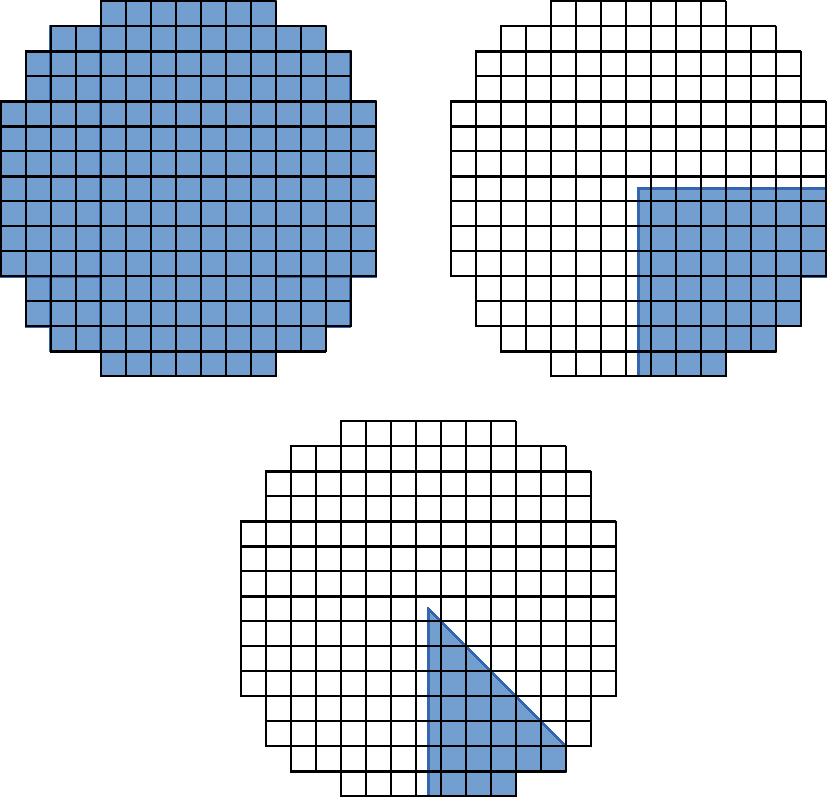
\includegraphics[width=5in]{figs/core_symmetry.pdf}
\end{center}
\caption{\label{fig:coresym} Full, quarter, and octant symmetry regions for a core map.}
\end{figure}

All of the maps require one entry for each assembly location defined in the {\it core\_shape} map.
However, the input parser can be used to take advantage of core symmetry.  If the core is symmetric,
the user only needs to input the maps in quarter or octant symmetry, and the input parser will automatically
unfold the map to full-symmetry.
The symmetry used in the core maps is independent of the symmetry used to run the actual calculations.
For example, the user can enter all of the core maps in octant symmetry and still run the calculations
in quarter or full symmetry.
The quadrant and octant that the parser is expecting is shown in Figure~\ref{fig:coresym}.

If there is an empty location in the map (e.g. if there is no detector or no control rod
in an assembly), enter a dash ``-'' for that location.  The dash is significant and signifies an
empty location in the core map.  (The dash represents something is missing, but it is still
a valid assembly location. The ``0'' in the {\it core\_shape} represents an invalid assembly location.)


\clearpage

The {\it assm\_map} shows where the assembly types are located within the core.
In the example below, there are three assembly types which will be defined in [ASSEMBLY] block(s).
\begin{verbatim}
  assm_map
                  A3 A3 A3 A3 A3 A3 A3
            A3 A3 A3 A1 A3 A1 A3 A1 A3 A3 A3
         A3 A3 A2 A1 A2 A1 A2 A1 A2 A1 A2 A3 A3
         A3 A2 A2 A2 A1 A2 A1 A2 A1 A2 A2 A2 A3
      A3 A3 A1 A2 A1 A2 A1 A2 A1 A2 A1 A2 A1 A3 A3
      A3 A1 A2 A1 A2 A1 A2 A1 A2 A1 A2 A1 A2 A1 A3
      A3 A3 A1 A2 A1 A2 A1 A2 A1 A2 A1 A2 A1 A3 A3
      A3 A1 A2 A1 A2 A1 A2 A1 A2 A1 A2 A1 A2 A1 A3
      A3 A3 A1 A2 A1 A2 A1 A2 A1 A2 A1 A2 A1 A3 A3
      A3 A1 A2 A1 A2 A1 A2 A1 A2 A1 A2 A1 A2 A1 A3
      A3 A3 A1 A2 A1 A2 A1 A2 A1 A2 A1 A2 A1 A3 A3
         A3 A2 A2 A2 A1 A2 A1 A2 A1 A2 A2 A2 A3
         A3 A3 A2 A1 A2 A1 A2 A1 A2 A1 A2 A3 A3
            A3 A3 A3 A1 A3 A1 A3 A1 A3 A3 A3
                  A3 A3 A3 A3 A3 A3 A3
\end{verbatim}

The following map is equivalent to the previous map, but demonstrates the use of input with octant symmetry.
Only values in the octant shown in Figure~\ref{fig:coresym} are entered in the map and the parser automatically
unfolds the map to full-symmetry.
\begin{verbatim}
  assm_map
     A1
     A2 A1
     A1 A2 A1
     A2 A1 A2 A1
     A1 A2 A1 A2 A2
     A2 A1 A2 A1 A2 A3
     A1 A3 A1 A3 A3 A3
     A3 A3 A3 A3         ! assembly map with octant symmetry
\end{verbatim}

The {\it insert\_map} is used to show where assembly inserts are located within the core.
In the following qtr-symmetry example,
the inserts are burnable poison assemblies with different numbers of pyrex rods.
The {\it insert\_map} can also be used to place geometry objects such as thimble plugs.
The geometry description of the inserts will be given in the [INSERT] block.
\vfill   % don't split map
\begin{verbatim}
  insert_map
      -    BP20   -    BP20   -    BP20   -    BP12
     BP20   -    BP24   -    BP20   -    BP24   -
      -    BP24   -    BP20   -    BP16   -    BP8
     BP20   -    BP20   -    BP20   -    BP16   -
      -    BP20   -    BP20   -    BP24   -
     BP20   -    BP16   -    BP24  BP12   -
      -    BP24   -    BP16   -     -
     BP12   -    BP8    -
\end{verbatim}
The {\it insert\_map} is optional if no inserts are present in the core.
A dash ``-'' is used to specify assembly locations without an insert.

The {\it det\_map} is used to show where detectors are located in the core.  The geometry description
of the corresponding detector strings is given in the [DETECTOR] block.  In this example,
there is only one detector type denoted with a ``1''.  Since the ``1'' occurs in a core map,
it is treated as a character string.  This example uses a full-symmetry map.
\begin{verbatim}
  det_map
                 -  -  1  -  -  1  -
           1  -  -  1  -  1  -  -  -  -  -
        -  -  -  -  -  -  1  -  1  -  1  -  1
        1  1  -  -  -  -  1  -  -  -  -  -  -
     -  -  -  -  1  -  -  -  1  -  1  -  1  -  -
     1  -  1  -  -  1  -  1  -  -  -  -  -  1  -
     -  -  -  1  -  -  1  -  -  1  -  -  1  -  -
     1  -  1  -  1  -  1  -  -  1  -  1  1  1  -
     -  1  -  -  -  -  -  -  1  -  1  -  -  -  1
     -  -  -  -  1  -  1  -  -  -  -  1  -  -  -
     1  -  -  -  1  -  -  1  -  -  1  -  -  -  1
        -  -  -  -  1  -  -  1  -  -  1  -  -
        -  1  -  1  -  -  1  -  -  -  -  -  1
           1  -  -  -  1  -  -  1  -  1  -
                 1  -  -  1  -  -  -
\end{verbatim}
The {\it det\_map} is optional if no detectors are present in the core.
A dash ``-'' is used to specify assembly locations without a detector.

% fix: Need to define what a control rod bank is

The control rod assemblies are described with two maps.  The {\it crd\_map}
defines the control rod types and locations in the core.
The {\it crd\_bank} map assigns control rod locations to control rod banks.
The control rod maps are optional if no control rods are present in the core.
In the following example, there is only one control rod type with label ``1''.
\vfill   % don't split map
\begin{verbatim}
  crd_map
                 -  -  -  -  -  -  -
           -  1  -  1  -  1  -  1  -  1  -
        -  -  -  1  -  1  -  1  -  1  -  -  -
        1  -  1  -  -  -  1  -  -  -  1  -  1
     -  -  1  -  1  -  -  -  -  -  1  -  1  -  -
     -  1  -  -  -  1  -  1  -  1  -  -  -  1  -
     -  -  1  -  -  -  -  -  -  -  -  -  1  -  -
     -  1  -  1  -  1  -  1  -  1  -  1  -  1  -
     -  -  1  -  -  -  -  -  -  -  -  -  1  -  -
     -  1  -  -  -  1  -  1  -  1  -  -  -  1  -
     -  -  1  -  1  -  -  -  -  -  1  -  1  -  -
        1  -  1  -  -  -  1  -  -  -  1  -  1
        -  -  -  1  -  1  -  1  -  1  -  -  -
           -  1  -  1  -  1  -  1  -  1  -
                 -  -  -  -  -  -  -
  crd_bank
                 -  -  -  -  -  -  -
           - SA  -  B  -  C  -  B  - SA  -
        -  -  - SD  - SB  - SB  - SC  -  -  -
       SA  -  D  -  -  -  D  -  -  -  D  - SA
     -  - SC  -  A  -  -  -  -  -  A  - SD  -  -
     -  B  -  -  -  C  -  A  -  C  -  -  -  B  -
     -  - SB  -  -  -  -  -  -  -  -  - SB  -  -
     -  C  -  D  -  A  -  D  -  A  -  D  -  C  -
     -  - SB  -  -  -  -  -  -  -  -  - SB  -  -
     -  B  -  -  -  C  -  A  -  C  -  -  -  B  -
     -  - SD  -  A  -  -  -  -  -  A  - SC  -  -
       SA  -  D  -  -  -  D  -  -  -  D  - SA
        -  -  - SC  - SB  - SB  - SD  -  -  -
           - SA  -  B  -  C  -  B  - SA  -
                 -  -  -  -  -  -  -

\end{verbatim}

%%%%%%%%%%%%%%%%%%%%%%%%%%%%%%%%%%%%%%%
\subsection{Core Baffle and Vessel}

The core baffle (sometimes called the shroud) is a steel reflector that closely surrounds
the fuel assemblies in the core. The barrel is a round steel structure that surrounds the baffle, and
the vessel is the round outer pressure vessel.  These structures are shown in
Figure~\ref{fig:corebaffle}.

\begin{figure}
\begin{center}
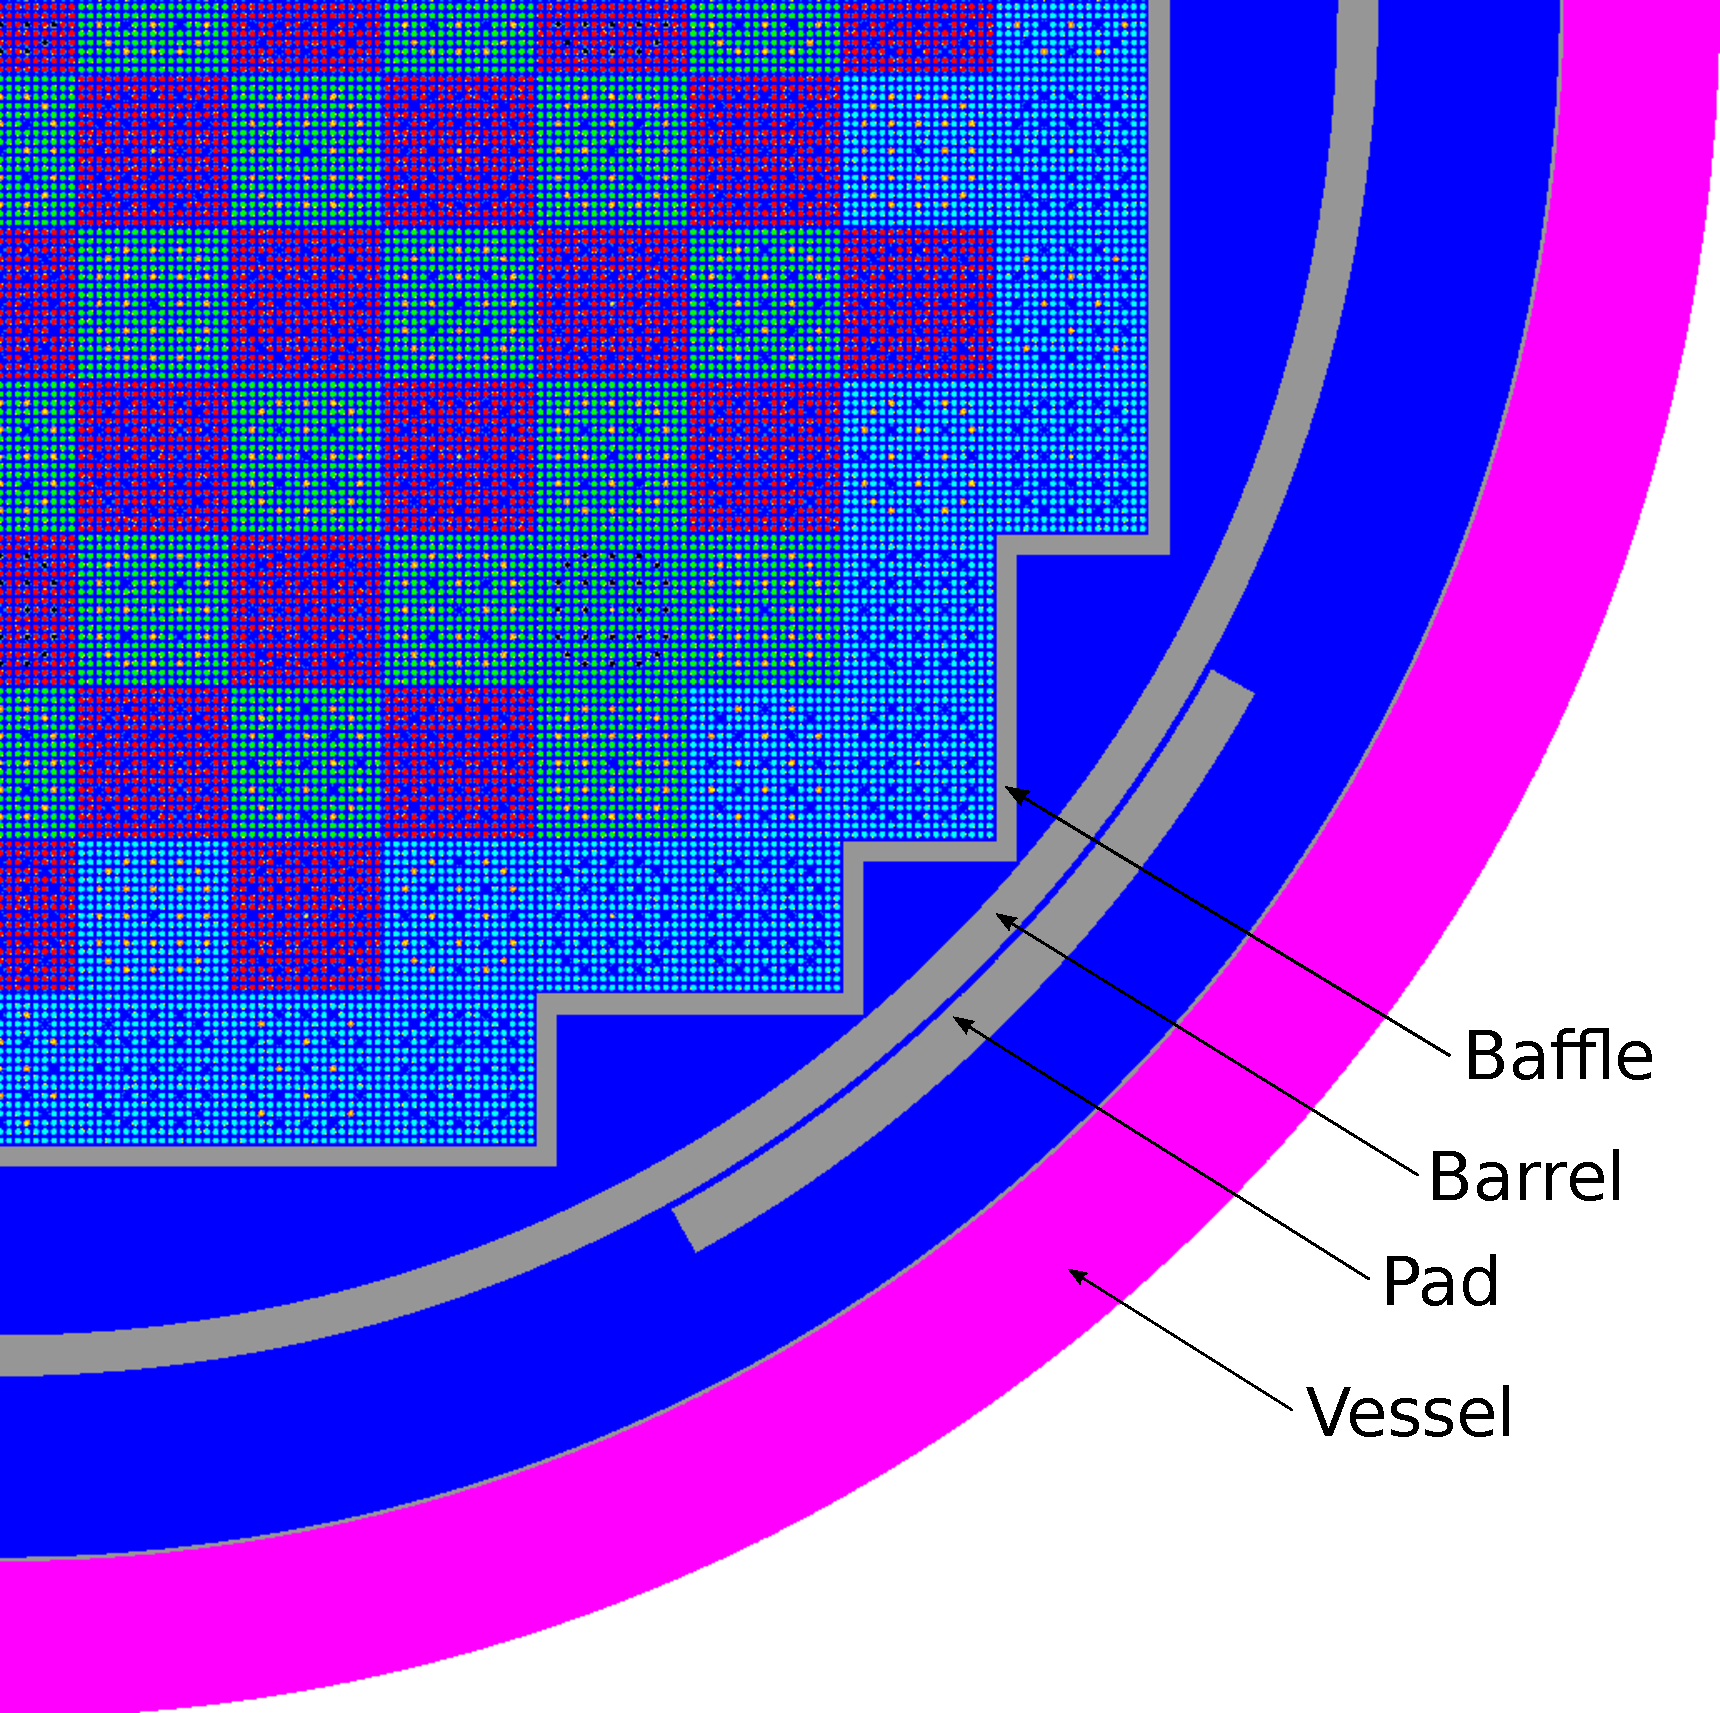
\includegraphics[width=5in]{figs/core_baffle.pdf}
\end{center}
\caption{\label{fig:corebaffle} Core baffle and vessel (image courtesy of Andrew Godfrey).}
\end{figure}

% fix: add figure showing exactly how the baffle gap is defined

The {\it baffle} is defined with a single material, the size of the gap between the
outer assembly and baffle, and the baffle thickness.
\begin{verbatim}
  baffle   SS304 0.19 1.26   ! material, gap (cm), and thickness (cm)
\end{verbatim}

The barrel and vessel are defined with a {\it vessel} card.  This card allows the
user to enter any arbitrary number of rings surrounding a core by specifying the
ring radii and the materials between the rings.

\begin{verbatim}
  vessel   mod 166.7 SS304 169.2 mod 175.0 SS304 176.0   ! materials and radii (cm)
\end{verbatim}

There is currently no input defined to specify the neutron pad.

%%%%%%%%%%%%%%%%%%%%%%%%%%%%%%%%%%%%%%%
\subsection{Core Plates}

The core plates are large steel plates at the top and bottom of the core that have
various flow holes passing through them.  All of the axial core heights are defined relative to the
top of the bottom core plate and the total core {\it height} is defined as the distance
between the top of the bottom core plate and the bottom of the top core plate.

The core plates are modeled in the neutronics codes as smeared materials.
The upper and lower core plates are defined with a material composition, a thickness, and a
volume fraction of the structural material.
The remainder of the volume fraction is filled with coolant.

\begin{verbatim}
  lower_plate SS304  5.0  0.5   ! material, thickness (cm), volume fraction
  upper_plate SS304  7.6  0.5   ! material, thickness (cm), volume fraction
\end{verbatim}

%%%%%%%%%%%%%%%%%%%%%%%%%%%%%%%%%%%%%%%
\subsection{Small Core Geometries}
\label{sec:smallcoregeom}

Even though the VERA input is designed for ``real'' core geometries, it can accommodate smaller
problems as well.
For example, if the user only wants to run a single-assembly calculation, they would define the core size
as one assembly by one assembly, and all of the core maps would contain a single assembly.
\begin{verbatim}
  size 1                ! core composed of a single-assembly
  core_shape
     1
\end{verbatim}

If the user wants to model a single fuel rod, they would define a core with one assembly and
an assembly with one rod in it.



%%%%%%%%%%%%%%%%%%%%%%%%%%%%%%%
%  Section: Assemblies
%*-------------------------------------------------------------------------*
%*                 Copyright 2013-2015 Core Physics, Inc.                  *
%*  Under terms of the contract to support CASL, there is a non-exclusive  *
%*  license for use of this work by or on behalf of the U.S. Government.   *
%*-------------------------------------------------------------------------*
%
% @version CVS $Id: assemblies.tex,v 1.23 2015/02/23 00:56:17 scott Exp $
%
%%%%%%%%%%%%%%%%%%%%%%%%%%%%%%%%%%%%%%%%%%%%%%%%%%%%%%%%%%%%%%%%
\section{Assembly Description}

The [ASSEMBLY] block contains the geometric description of a unique fuel assembly design (type).
Multiple [ASSEMBLY] blocks are allowed to describe different assembly designs in the core.

If there are multiple assembly designs that are geometrically identical (i.e. everything is the same except
the enrichments), then they can all be defined in a single [ASSEMBLY] block.
Each assembly type will have a unique {\it axial} card with possibly unique axial levels and lattice types.
Assemblies within a single reload typically have a design similar enough that they can share a single
[ASSEMBLY] block.

If assembly designs are not geometrically identical (e.g. different vendors, different generations, etc.)
they need to be defined in separate [ASSEMBLY] blocks.
One advantage to having separate blocks for each assembly design is that each design can be
modeled (and archived) independently without having to rely on global definitions.

A typical PWR assembly is shown in Figure~\ref{fig:assembly}.  Refer to this figure in the following discussions.
\begin{figure}
\begin{center}
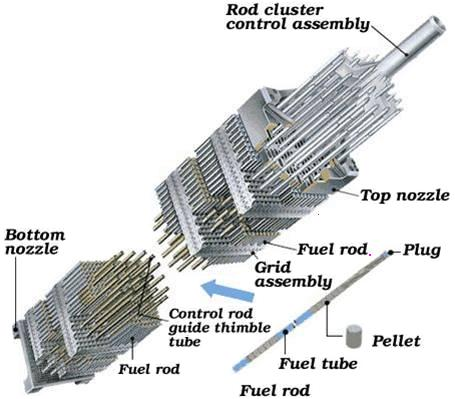
\includegraphics[width=4in]{figs/PWR-assembly.jpg}
\end{center}
\caption{\label{fig:assembly} PWR Fuel Assembly (source: Public internet).}
\end{figure}

A complete listing of all the input cards in the [ASSEMBLY] block is located in Section~\ref{sec:assemblycards}.

%%%%%%%%%%%%%%%%%%%%%%%%%%%
\subsection{Initial Data}

Each assembly block must contain a geometry description with the number of pins across the assembly and
the pin pitch.  An assembly block can also include an optional title card.
\begin{verbatim}
  title "Westinghouse 17x17"      ! assembly title
  npin 17                         ! number of pins across one side
  ppitch 1.260                    ! pin pitch (cm)
\end{verbatim}

The number of pins {\it npin} must be the same for every assembly in a core.

The inter-assembly gap on each side of the assembly is calculated as $[apitch-npin*ppitch]/2$

The fuel and structural materials are defined with the following cards.
See Chapter~\ref{chap:materials} for a complete description of the material inputs.
\begin{verbatim}
  fuel U31 10.257 95.0 / 3.1   ! mat, density (g/cc), Theoretical density (%)
                               !    / U-235 enrichment (%)
  mat inc   8.19               ! mat, density (g/cc)
  mat ss    8.0
  mat zirc4 6.56
\end{verbatim}

%%%%%%%%%%%%%%%%%%%%%%%%%%%
\subsection{Cell Descriptions}

Cell cards are used to describe ``pincells''.  A pincell is defined as a configuration
of concentric cylinders (or rings) centered in a square region of coolant.
Cell configurations can be used to model fuel rods or guide tubes,
as shown in Figure~\ref{fig:pincell}.
\begin{figure}
\begin{center}
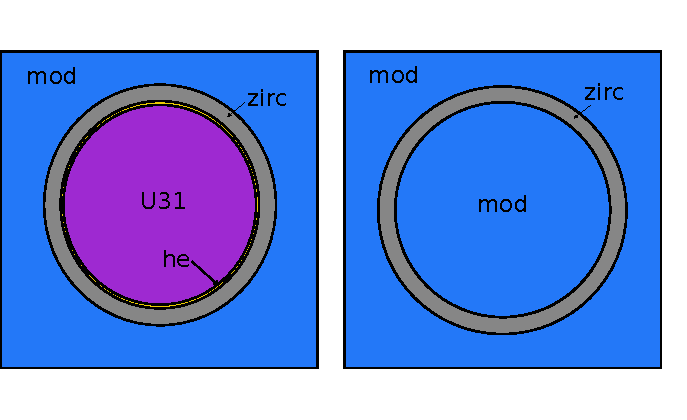
\includegraphics[width=4in]{figs/pincell1.pdf}
\end{center}
\caption{\label{fig:pincell} Pincell diagrams of a fuel rod and a guide tube.}
\end{figure}

The first parameter on the {\it cell} card is the cell ID.
This is followed by a list of radii for each ring in the cell, followed by a slash.
After the slash is a list of materials that compose each ring.
The cell ID's are used in the rod maps described in the next section.

\begin{verbatim}
  cell 1     0.4096 0.418 0.475 / U31 he zirc4
  cell GT           0.561 0.602 / mod    zirc4      ! guide tube
  cell IT           0.561 0.602 / mod    zirc4      ! instrument tube
  cell 7            0.418 0.475 / mod    mod        ! empty location
  cell 8            0.418 0.475 /     he zirc4      ! plenum
  cell 9                  0.475 /        zirc4      ! pincap
\end{verbatim}

In this example, in cell ``1'', the material ``U31'' extends from radius 0 to 0.4096.
The material ``he'' extends from a radius 0.4096 to 0.418.
The materials ``U31'' and ``he'' are defined on {\it fuel} and {\it mat} cards, respectively.
(Refer to Chapter~\ref{chap:materials} for a complete description on defining materials.)

The outside of each cell is automatically filled with the special material ``mod'', which
refers to the moderator (or coolant).
The composition of ``mod'' is calculated by the codes using the local T/H conditions and the
soluble boron concentration, and cannot be specified by a user on a {\it mat} card.

In the example above, the guide tube (GT) and instrument tube (IT) descriptions
use the special moderator material ``mod'' to define the moderator material on both
the inside and outside of the tubes.

Note that large water rods that span more than one lattice cell are not currently supported in the input
(e.g. large CE water rods that span four lattice cells).
In the future, an option will be added to the {\it cell} card to specify if a water rod spans more than one cell. 

%%%%%%%%%%%%%%%%%%%%%%%%%%%
\subsection{Lattice Descriptions}

Once the cells are defined, they are placed into 2D ``lattices'' as shown below.
Like the core maps, the lattice maps can be entered with either full-symmetry, qtr-symmetry,
or octant-symmetry.  The maps below are octant symmetric maps for 17x17 assembly designs.
\vfill   % don't split map
\begin{verbatim}
  rodmap FUEL1
      IT
       1 1
       1 1 1
      GT 1 1 GT
       1 1 1  1 1
       1 1 1  1 1 GT
      GT 1 1 GT 1  1 1
       1 1 1  1 1  1 1 1
       1 1 1  1 1  1 1 1 1

  rodmap LGAP1
      IT
       7 7
       7 7 7
      GT 7 7 GT
       7 7 7  7 7
       7 7 7  7 7 GT
      GT 7 7 GT 7  7 7
       7 7 7  7 7  7 7 7
       7 7 7  7 7  7 7 7 7

  rodmap PLEN1
      IT
       8 8
       8 8 8
      GT 8 8 GT
       8 8 8  8 8
       8 8 8  8 8 GT
      GT 8 8 GT 8  8 8
       8 8 8  8 8  8 8 8
       8 8 8  8 8  8 8 8 8

  rodmap PCAP1
      IT
       9 9
       9 9 9
      GT 9 9 GT
       9 9 9  9 9
       9 9 9  9 9 GT
      GT 9 9 GT 9  9 9
       9 9 9  9 9  9 9 9
       9 9 9  9 9  9 9 9 9
\end{verbatim}

Rod maps define each unique axial level in the assembly.
The first parameter is the lattice name (e.g. FUEL1, PCAP1, etc.),
followed by a map of the {\it cell} ID's.

Each entry in a rod map must be a valid cell ID.

%%%%%%%%%%%%%%%%%%%%%%%%%%%
\subsection{Axial Descriptions}

After rod maps are defined for each axial level, the lattices are ``stacked'' into
an assembly using an {\it axial} card as shown below.

\begin{verbatim}
  axial A1    6.050
      LGAP1  10.281
      PCAP1  11.951
      FUEL1 377.711
      PLEN1 393.711
      PCAP1 395.381
      LGAP1 397.501
\end{verbatim}

The {\it axial} card tells the code how to place the lattices axially.
The first parameter is the name of the assembly (A1), followed by a
list of elevations and lattice types.
For example, lattice ``FUEL1'' extends from 11.951 to 377.711 cm axially.

Multiple assembly types can be defined in a single [ASSEMBLY] block by using
multiple {\it axial} cards, each with a unique assembly ID.

All axial elevations are defined relative to the top of the lower core plate.

%%%%%%%%%%%%%%%%%%%%%%%%%%%
\subsection{Grid Spacer Descriptions}

Grid cards are used to define unique grid spacer types.
The following example defines two grid types, ``END'' and ``MID''.
\begin{verbatim}
  grid END inc   1017  3.866   ! grid spacer material, mass(g), height(cm)
  grid MID zirc4  875  3.810
\end{verbatim}

The grid types are placed axially with the {\it grid\_axial} card:
\vfill   % don't split map
\begin{verbatim}
  grid_axial
      END  13.884
      MID  75.2
      MID 127.4
      MID 179.6
      MID 231.8
      MID 284.0
      MID 336.2
      END 388.2
\end{verbatim}

The elevations are the midpoints of the spacer grid and are relative to the top of the lower core plate.

%%%%%%%%%%%%%%%%%%%%%%%%%%%
\subsection{Nozzle Descriptions}

The assembly nozzles are modeled in the neutronics codes as smeared materials.  This is a very good
approximation since the nozzles are not in the active fuel region and are mostly
composed of water, steel, and zirconium.  The user only specifies a nozzle mass and a nozzle height.
The total volume of the nozzle region is calculated from the assembly pitch and nozzle height.
The volume of the nozzle is calculated from the nozzle mass and density.
The volume of the coolant is then calculated as the total volume minus the volume of the nozzle.
The coolant density is updated with the local T/H conditions.

% A typical PWR assembly nozzle is shown in Figure~\ref{fig:nozzle}.
% \begin{figure}
% \begin{center}
% 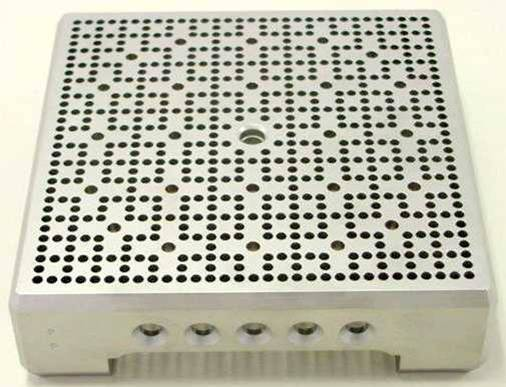
\includegraphics[width=4in]{figs/nozzle.jpg}
% \end{center}
% \caption{\label{fig:nozzle} PWR Assembly Lower Nozzle.}
% \end{figure}

\begin{verbatim}
  lower_nozzle  ss 6.05  6250.0  ! mat, height (cm), mass (g)
  upper_nozzle  ss 8.827 6250.0  ! mat, height (cm), mass (g)
\end{verbatim}

Only a single material can be specified on a nozzle card.  If the user wants to use
more than one material to define a nozzle, they can define a custom material that
is a mixture of the materials and then use the custom material in the nozzle card.

Note that the {\it lower\_nozzle} height should match the bottom elevation on the {\it axial} card.
The {\it upper\_nozzle} height + the top elevation on the {\it axial} card must match the
core {\it height} in the [CORE] block.
The input parser does not currently perform a check to make sure the elevations are consistent.
Therefore, this check should be performed in each of the individual physics codes.

%%%%%%%%%%%%%%%%%%%%%%%%%%%%%%%%%%%%%%%%%%%%%%%%%%%%%%%%%%%
\section{Control Rod Assembly Description}

The [CONTROL] block contains the geometric description of a control assembly.

A control rod assembly is defined in the same way that a fuel assembly is defined.
The user specifies cells, lattices, and axial descriptions of the control rod assembly. 
The main difference between the control rod assembly and the fuel assembly is that
the control rod assembly describes what is inside the guide tubes and the fuel assembly
defines the guide tubes themselves.

Control rod positions change during operation, so the geometric description of a control rod
should always be for a rod in the {\bf fully inserted} position.
In the example below, the bottom of the control rod in the fully inserted position is 
at an axial location of 15.46 cm.

\begin{verbatim}
  title "B4C control rods with AIC tips" 
  npin 17

  cell 1  0.382 0.386 0.484 / aic he ss      ! AIC cell
  cell 2  0.373 0.386 0.484 / b4c he ss      ! B4C cell

  rodmap  AIC
     -
     - -
     - - -
     1 - - 1
     - - - - -
     - - - - - 1
     1 - - 1 - - -
     - - - - - - - -
     - - - - - - - - -

  rodmap  B4C
     -
     - -
     - - -
     2 - - 2
     - - - - -
     - - - - - 2
     2 - - 2 - - -
     - - - - - - - -
     - - - - - - - - -

  axial CR1 15.46 AIC  376.44 B4C  394.3
\end{verbatim}

The name of the control rod ``CR1'' refers to the control rod type in the
{\it crd\_map} in the [CORE] block.

Control rods positions are assigned to a control rod bank with the {\it crd\_bank} map
in the [CORE] block, and then the banks are positioned with the 
{\it rodbank} card in the [STATE] block.

Note that the locations of the control rod fingers must match the guide tube locations in the
corresponding [ASSEMBLY] block descriptions.  Furthermore, the outer radii of the control
rod fingers must be smaller than the inner radii of the guide tubes.
The input parser does not currently perform a check to make sure the control rod finger
descriptions are consistent with the guide tube descriptions.
This check should be performed in each of the individual physics codes.

The user can define materials in the [CONTROL] block.  These materials only have scope in
this block and are not accessible by other blocks.  See Chapter~\ref{chap:materials} for details.

A complete listing of all the input cards in the [CONTROL] block is located in Section~\ref{sec:controlcards}.

%%%%%%%%%%%%%%%%%%%%%%%%%%%
\subsection{Control Rod Stroke}
\label{sec:stroke}

The difference between control rod descriptions and assembly descriptions is that
the control rods move during operation.  This movement is defined with a {\it stroke} card.

The first value on the {\it stroke} card is the total length of the control rod travel (stroke)
from fully inserted to fully withdrawn.

The second value on the {\it stroke} card is the number of steps in the fully withdrawn position.
Step 0 is the fully inserted position.  The number of steps in the fully withdrawn position 
is specified by the user, but 228 steps is often used for typical Westinghouse PWR's.
\begin{verbatim}
  stroke  360.0 228      ! stroke (cm), number of steps fully withdrawn
\end{verbatim}

To position the control rods in percent withdrawn (\%), the number of steps should be set to 100 and
each step will signify 1\% withdrawn.

The geometry description in the input is for a control rod in the fully inserted position (step 0).

\subsection{Control Rod Position Example}

From the {\it axial} card shown above, the bottom of the AIC at the fully-inserted position is 15.46 cm.
From the {\it stroke} card, the total stroke is 360.0 cm and the number of steps in the fully withdrawn
position is 228 steps.
Therefore, the bottom elevation of the AIC lattice at step N will be
\begin{equation}
   E(N) = 15.46 + \frac{360.0 \cdot N}{228}
\end{equation}

Using this formula, the bottom elevation of the AIC lattice at the following step positions is:
\begin{itemize}   % itemize = bullet list
 \item step 228 (fully withdrawn)= 15.46 + 360.0 * 228 / 228 = 375.46 cm
 \item step 100 = 15.46 + 360.0 * 100 / 228 = 173.35 cm
 \item step 0 (fully inserted) = 15.46 + 360.0 * 0 / 228 = 15.46 cm
\end{itemize}

%%%%%%%%%%%%%%%%%%%%%%%%%%%%%%%%%%%%%%
\section{Insert Description}
An assembly insert is defined in the same way as a fuel assembly or control rod assembly is defined.
The user defines the insert using cells, lattices, and axial descriptions.

The fuel assembly description should contain the guide tube descriptions and the insert description
defines what is inserted in the guide tubes.  Assembly inserts can be inserted and withdrawn
during a core shuffle (by specifying a {\it insert\_map} card in the [CORE] block),
but cannot be moved during a cycle depletion.

The insert and control rod descriptions are very similar, with the only difference being that the
insert cannot change position axially during a cycle depletion and a control rod moves axially
during operations.

The following example shows a definition of a Pyrex insert.

\begin{verbatim}
[INSERT]
    title "Pyrex"
    npin 17
    mat pyrx1 2.25 pyrex-vera
    cell 1  0.214 0.231 0.241 0.427 0.437 0.484 / he ss he pyrx1 he ss
    rodmap  PY24
       -
       - -
       - - -
       1 - - 1
       - - - - -
       - - - - - 1
       1 - - 1 - - -
       - - - - - - - -
       - - - - - - - - -

    axial INS24  15.76 PY24 376.441
\end{verbatim}

The name of the insert ``INS24'' refers to an insert type defined in the
{\it insert\_map} in the [CORE] block.

The locations of the insert fingers must match the guide tube locations in the
corresponding [ASSEMBLY] block descriptions.  In addition, the outer radii of the insert
fingers must be smaller than the inner radii of the guide tubes.
The input parser does not currently perform a check to make sure the insert finger
descriptions are consistent with the guide tube descriptions.
This check should be performed in each of the individual physics codes.

As with [ASSEMBLY] blocks, multiple insert types can be defined in a single [INSERT]
block by using multiple {\it axial} cards, each with a unique insert ID.

A complete listing of all the input cards in the [INSERT] block is located in Section~\ref{sec:insertcards}.

%%%%%%%%%%%%%%%%%%%%%%%%%%%%%%%%%%%%%%
\section{Detector Description}
A detector string is defined in the same way that a fuel assembly or insert assembly is defined.
The user defines cells, lattices, and axial descriptions for the detector string.

The insert and detector descriptions are very similar, with the difference being that
detectors have special properties used to calculate instrumentation signals.

\begin{verbatim}
  [DETECTOR]
    title "Incore instrument thimble"
    npin 17

    mat he 0.0001786
    mat ss 8.0

    cell 1  0.258 0.382 / he ss

    rodmap  LAT
       1
       - -
       - - -
       - - - -
       - - - - -
       - - - - - -
       - - - - - - -
       - - - - - - - -
       - - - - - - - - -

    axial D1  0.0 LAT 406.337
\end{verbatim}

The name of the detector ``D1'' refers to a detector type defined in the
{\it det\_map} in the [CORE] block.

A complete listing of all the input cards in the [DETECTOR] block is located in Section~\ref{sec:detectorcards}.





%%%%%%%%%%%%%%%%%%%%%%%%%%%%%%%
%  Section: State
%*-------------------------------------------------------------------------*
%*                 Copyright 2013-2015 Core Physics, Inc.                  *
%*  Under terms of the contract to support CASL, there is a non-exclusive  *
%*  license for use of this work by or on behalf of the U.S. Government.   *
%*-------------------------------------------------------------------------*
%
% @version CVS $Id: state.tex,v 1.5 2015/02/17 03:26:30 Scott Exp $
%
%%%%%%%%%%%%%%%%%%%%%%%%%%%%%%%%%%%%%%%%%%%%%%%%%%%%%%%%%%%%%%%%
\section{State Description}

The [STATE] block defines the state of the core
(power, flow, pressure, inlet temperature, rod positions, boron concentration, etc.)
at a particular point in time.
These values will typically change during a cycle depletion.

An example showing the most common input cards in the [STATE] block is shown below.
A complete listing of all the input cards in the [STATE] block is located in Section~\ref{sec:statecards}.

\begin{verbatim}
  [STATE]
    power   98.0       ! % of rated power - rated values defined in [CORE] block
    flow   100.0       ! % of rated flow
    pressure 2250.0    ! psia
    tinlet 557.33 F    !
    feedback on        ! turn on T/H feedback

    boron   1285       ! initial boron ppmB
    search  boron      ! turn on boron search

    sym qtr            ! run problem in qtr-symmetry

    rodbank SA 228
            SB 228
            SC 228
            SD 228
             A 228
             B 228
             C 228
             D 167
\end{verbatim}

The {\it sym} card tells the code to run the calculation in full-core or
qtr-core symmetry. If the calculation is run in qtr-core symmetry, the symmetry is either
set to qtr-core rotational or qtr-core mirror by the {\it bc\_sym} card in the [CORE] block.

The {\it rodbank} card is used to position the control rods. The {\it rodbank} input includes pairs of bank names
and bank positions.  The bank names correspond to the {\it crd\_map} in the [CORE] block.
The positions indicate the position of the control rod bank in steps.
Step 0 is fully inserted.
The number of steps for a rod to be completely withdrawn is set by the {\it stroke} card in
the [CONTROL] block (see Section~\ref{sec:stroke}). For Westinghouse PWR's, a typical value of fully-withdrawn is 228 steps.

%%%%%%%%%%%%%%%%%%%%%%%%%%%%%%%
\section{Edits Description}

The [EDITS] block is used to control the output edits.

One of the edits produced by the core simulator is the rod power.   The user has 
the ability to specify the axial levels that the power is averaged over with 
the {\it axial\_edit\_bounds} card.
The user may choose to average power over uniform axial intervals (like most nodal codes),
or to specify the edit intervals manually.

(Note: the edit options are under development and more options will be added in the future.)

A complete listing of all the input cards in the [EDITS] block is located in Section~\ref{sec:editscards}.

\subsection{COBRA-TF Nodalization}

The {\it axial\_edit\_bounds} card is also used to set the axial nodalization when coupling
the neutronics physics code to the COBRA-TF (CTF) subchannel code.

When running CTF, there is a restriction that the grid boundaries must be explicitly
included in the {\it axial\_edit\_bounds}. This can get a little complicated for the user.
In the VERA input, spacer grids are defined in the [ASSEMBLY] block by specifying the 
grid heights on the {\it grid} card and the elevations of the grid midpoints 
on the {\it grid\_axial} card.
From the grid heights and midpoints, the elevations at the top and bottom of the spacer grid
can be calculated, and then the top and bottom elevations must be included 
in the {\it axial\_edit\_bounds}.

For example, if a grid is defined with a centerline at 75.0 and a height of 2.5, then the
{\it axial\_edit\_bounds} must include the points $75.0 \pm 1.25 = 73.75$ and $76.25$.

\begin{verbatim}
   [ASSEMBLY]
    grid GRID1 inc 1000 2.5    ! grid name, material, mass (g), and height (cm)
    grid_axial                 ! locations of grid midpoints (cm)
        GRID1 75.0

   [EDITS]
    axial_edit_bounds
       ...
       73.75           ! this array must include top and bottom grid boundaries
       76.25
       ...
\end{verbatim}

The reason for this restriction is because the power is already calculated on the {\it axial\_edit\_bounds},
so it is natural to use the same power distribution to couple to the CTF model as well.
The grids must be explicitly included in the CTF boundaries so the loss coefficients are calculated correctly.

In the future, this restriction may be lifted and an additional edit bounds array may
be added explicitly for CTF calculations.


%%%%%%%%%%%%%%%%%%%%%%%%%%%%%%%
\section{Coupling Description}

The [COUPLING] block defines the relaxation parameters and convergence criteria to be
used when coupling different physics codes.  These values are used to determine
convergence {\it between} physics codes.  Convergence criteria {\it within} a physics
code is controlled by the code-specific block.

Refer to Section~\ref{sec:couplingcards} for a complete listing of all the cards in the [COUPLING] block.

No code-specific information is included in the [COUPLING] block.  All code-specific information
is contained in the code-specific blocks.  The [COUPLING] block is only used to define
generic coupling parameters.

As an example, consider the following multi-physics code coupling:
\begin{enumerate}
  \item  Run T/H calculation
  \item  Run neutronics calculation
  \item  Check eigenvalue convergence \label{stepepsk}
  \item  Check power convergence \label{stepepsp}
  \item  Relax/dampen the power shape
  \item  If not converged, go to step 1.
\end{enumerate}
The eigenvalue convergence in step~\ref{stepepsk} uses the card {\it epsk} to check
the change in eigenvalue between coupled iterations.
There are additional eigenvalue convergence criteria {\it within} the neutronics
code, but the internal parameters are specified in the individual code blocks.

The power convergence in step~\ref{stepepsp} uses the card {\it epsp} to check
the change in power between coupled iterations.

Additional convergence checks are made on the peak fuel temperature, maximum change in density,
and change in boron concentration (if applicable).

The example shown above uses a Picard iteration to converge.  Picard iterations usually
need to apply a relaxation factor (also called a damping factor or under-relaxation factor) to
one or more of the calculated quantities to converge.
The relaxation factors are applied in the following manner:
\begin{equation}
  x = \omega \, x^{\mbox{new}} + (1 - \omega) x^{\mbox{old}}
\end{equation}
where $x$ is the calculated parameter and $\omega$ is the relaxation factor.
A relaxation factor of 1.0 signifies no relaxation is performed.
A relaxation factor $< 1.0$ signifies under-relaxation.

Relaxation factors can be specified for the point-wise power, point-wise temperature, and/or point-wise density.
The relaxation is applied to the transferred quantities sent between physics codes.  The state variables
within each physics code are not changed.

An example [COUPLING] input block is shown below.

\begin{verbatim}
   [COUPLING]
     epsk        5.0  ! eigenvalue convergence (pcm)
     eps_temp    1.0  ! temperature convergence (deg C)
     eps_boron   0.1  ! boron convergence (ppm)
     rlx_power   0.5  ! power relaxation factor
     rlx_tfuel   1.0  ! fuel temperature relaxation factor
     rlx_den     1.0  ! density relaxation factor
     maxiter     20   ! maximum number of coupled iterations
\end{verbatim}

A complete listing of all the input cards in the [COUPLING] block is located in Section~\ref{sec:couplingcards}.



%%%%%%%%%%%%%%%%%%%%%%%%%%%%%%%%%%%%%%%%%
%  Chapter: Materials
%*-------------------------------------------------------------------------*
%*                 Copyright 2013-2015 Core Physics, Inc.                  *
%*  Under terms of the contract to support CASL, there is a non-exclusive  *
%*  license for use of this work by or on behalf of the U.S. Government.   *
%*-------------------------------------------------------------------------*
%
% @version CVS $Id: materials.tex,v 1.22 2015/02/23 00:56:17 scott Exp $
%
%%%%%%%%%%%%%%%%%%%%%%%%%%%%%%%%%%%%%%%%%
\chapter{Materials}  \label{chap:materials}

This chapter contains a description of the material input.  There are two types of materials
in the input file -- structural materials (input with a {\it mat} card) and fuel materials
(input with a {\it fuel} card).

Structural materials can be defined in either the [CORE] block, or in the
geometry object blocks [ASSEMBLY], [INSERT], [CONTROL], and [DETECTOR].
If the materials are defined in the [CORE] block, they have global scope.
If the materials are defined in the geometry object blocks, they only have
scope in the block they are defined.
The reason for this is to maintain the modularity of the geometry objects.

Fuel materials can only be defined in [ASSEMBLY] blocks.

Materials are used in many different input cards.  They are used to define
cells, nozzles, core plates, baffles, grids, reflectors, etc.  Every material that
is used in the input must be defined with either a {\it mat} card or a {\it fuel} card.

%%%%%%%%%%%%%%%%%%%%%%%%%%%%%%%%
\section{Structural Materials}

Structural materials are not fuel and do not deplete.  Structural
materials are defined with the following input card:

{\bf mat} {\it user-mat} {\it density} ({\it library-name$_i$}, {\it frac$_i$}, i=1, I)

where:
\begin{itemize}
\item {\it user-mat} is a user-defined material name.  It is case sensitive.  {\it user-mat} is used to
define material names in other input cards such as {\it cell}, {\it grid}, {\it nozzle}, etc. (No default)
\item {\it density} is the material density in g/cc (No default)
\item {\it library-name} is a corresponding material library name(s) for the user material.  The library name
must be defined in the material composition file. (Default = {\it user-mat}).  Multiple library materials
can be mixed to form a single user material.
\item {\it frac}  is the fraction of the library material in the user material. (Default=1.0 if there is only one library material in the user material).
\end{itemize}

There are two special user materials,  ``mod'' and ``vacuum''.
The user can use these materials in cell definitions, but the code will automatically
determine the composition of these materials  based on T/H feedback and soluble boron concentrations.
The user is not allowed to define a user material named ``mod'' or ``vacuum'' on a {\it mat} card.

The material libraries are code-specific libraries.  Please refer to the specific physics codes to
determine which library materials are available.

Some example material cards are shown below.
\begin{verbatim}
  mat zirc4 6.56                   ! library-name defaults to user-name 
  mat zirx  6.56 zirc4 1.0         ! user-name does not equal to library-name
  mat B10   12.0 boron 1.0
  mat XYZ   6.0  zirc4 0.8 ss 0.2  ! define new mixture of 80% zirc4 and 20% ss
  mat ABCD  8.0  zirc4 0.8 ss 0.15 b4c 0.05
\end{verbatim}

%% Fixed bug Andrew found below ~Feb 2014, atomic and weight were switched
All of the material fractions must sum to either +1.0 or -1.0.
If positive fractions are used, the fractions refer to weight fractions.
If negative fractions are used, the fractions refer to atomic fractions.

%%%%%%%%%%%%%%%%%%%%%%
\subsection{Search Order}

Structural materials can be defined in either the [CORE] block or one of the
geometry object blocks.  When a material is referred to in a block, it will look
for the material definition in the following order:
\begin{enumerate}  % enumerate = numbered list
 \item The code will first look for the material name in the local block ([ASSEMBLY], [INSERT], [CONTROL], or [DETECTOR])
 \item If the material is not found in the local block, it will look in the [CORE] block
\end{enumerate}

If materials are defined in the [CORE] block, they have global scope over the entire input.
If materials are defined in other blocks, they only have scope over the local block.  This means
that two geometry object blocks can use different material definitions with the same name.
One example of this is that two assemblies can be defined with the material ``zirc'', but
the ``zirc'' can have different compositions in each of the assemblies.

%%%%%%%%%%%%%%%%%%%%%%%%%%
\section{Composition File}

When using Shift all library materials must be included in a material composition file.
The composition file is a code-specific file which contains a list of all
of the available library materials.

Examples of typical library materials that are present on the composition file include:
\begin{itemize}   % itemize = bullet list
  \item aic (silver-indium-cadmium)
  \item b4c (boron carbide)
  \item boron
  \item inc (Inconel)
  \item he  (helium)
  \item ss  (stainless steel)
  \item zirc4 (Zircaloy-4)
\end{itemize}
Refer to the code-specific composition file for a complete list of valid library materials.

%%%%%%%%%%%%%%%%%%%%%%%%
\section{Fuel Materials}

Fuel materials are defined with {\it fuel} cards.
Fuel materials are heavy metal oxides which are usually UO$_2$ with different U-235 enrichments.
Fuel materials may also include MOX fuel, which consists of mixtures of uranium, plutonium and other actinides.
Fuel materials are different from structural materials in that they deplete and have
additional properties as described below.

Fuel can only be defined in [ASSEMBLY] blocks, and fuel materials can only be referenced by {\it cell} cards
in the [ASSEMBLY] block they are defined in.

Fuel materials are defined with the following input card:

{\bf fuel} {\it user-mat} {\it density} {\it thden} / {\it U-235\_enrichment}
    \{{\it HM\_material$_i$}={\it HM\_enrichment$_i$}, i=1, N\}  \\
   \{ / {\it gad\_material}={\it gad\_fraction} \}

Where:

\begin{itemize}   % itemize = bullet list
  \item {\it user-mat} is a user-defined fuel name. It is case sensitive. (No default)
  \item {\it density} is the fuel material density in g/cc (No default).
     The density is used to calculate number densities.
  \item {\it thden} is the percent of theoretical density in the pellet (\%) (No default).
   The theoretical density is only used to look up material properties in the fuel performance,
   it is not used to calculate number densities.  There is no ``double counting'' between
   {\it density} and {\it thden}.
  \item {\it U-235\_enrichment} is the U-235 enrichment in the fuel in weight \%  (No default).
  \begin{itemize}   % itemize = bullet list
    \item If U-234 and U-236 are not specified, they will automatically be added to the
       fuel by a pre-determined function (see below)
    \item If the sum of the heavy metal (HM) enrichments does not equal 100\%, the remainder of the
        HM composition will be assigned to U-238.
  \end{itemize}
  \item {\it HM\_material$_i$} is the material name for HM isotope $i$ (Pu-239, Pu-241, etc.) (optional) 
    The names of the HM materials must be valid library-names.
  \item {\it HM\_enrichment$_i$} is the enrichment of HM isotope $i$ in weight \% (optional)
  \item {\it gad\_material} is the material name for the gadolina oxide (or other material) (optional).
        The gad material is usually a mixture defined on a separate {\it mat} card.
  \item {\it gad\_fraction} is the weight percent of the gad material relative to the total fuel mass (optional)
\end{itemize}

Oxygen should not be included on the {\it fuel} card.  The correct amount of oxygen will automatically
be added to the HM to create an oxide (either UO$_2$  or (HM)O$_2$).

The {\it density} is the ``stack density'' or ``smeared density'' and should include the volume
of the pellet dishing and chamfers.
It is calculated as the total mass of the fuel pellets divided by the total volume of the fuel
\begin{equation}
  \mbox{stack density} = \frac{ (\mbox{fuel mass})} { \pi (\mbox{pellet radius})^2 \, (\mbox{fuel height}) }
\end{equation}

The {\it thden} refers to the actual theoretical density of the pellet.  This quantity is
used in fuel performance codes to evaluate material properties.

If U-234 or U-236 enrichments are not included in the fuel definition, they are automatically
added to the fuel with the following formulas:
\begin{equation}
   W_{234} = 0.007731 \cdot W_{235}^{1.0837}
\end{equation}
\begin{equation}
  W_{236} = 0.0046 \cdot W_{235}
\end{equation}
Where $W_{23x}$ is the enrichment of each of the uranium isotopes in percent.

If a user specifically does NOT want U-234 or U-236, they should specify a U-234 
and/or U-236 enrichment of zero.

Examples of typical {\it fuel} cards are shown below.  The user
only has to specify the U-235 enrichment and the code will automatically add
U-234, U-236, U-238, and oxygen to the fuel.
\begin{verbatim}
  fuel U21 10.4 95.2 / 2.1        ! 2.1% enriched UO2 fuel, no gad
  fuel UO2-35 10.297 95.0 / 3.5   ! 3.5% enriched UO2 fuel, no gad
  fuel U23    10.111 / 2.3        ! fuel with default thden
\end{verbatim}

An example of a {\it fuel} card with gadolinia burnable poison is shown next.
In this example, the gadolinia oxide is first defined with a {\it mat} card and 
is mixed with the fuel as 5\%  gad oxide and 95\% UO$_2$ (weight percents). 
\begin{verbatim}
  mat gad5 7.407 gd2o3 1.0                ! define gad material separately
  fuel U49 10.111 94.5 / 1.8  / gad5=0.05 ! 1.8% enriched fuel with 5% gad
\end{verbatim}

Some examples of MOX fuel cards are shown next.  In these cards, the user specifies
the U-235 enrichment (the U-235 enrichment is usually small in MOX fuel) and the
plutonium isotope enrichments.  The code will automatically add U-234, U-236, U-238,
and oxygen.
\begin{verbatim}
  fuel PX1  10.111 94.5 / 0.711 Pu-239=23.4 Pu-241=1.9    ! Sample MOX fuel
  fuel MOX1 10.111 94.5 / 1.0   Pu-238=1.0  Pu-239=26.0 
                    Pu-240=12.0 Pu-241=8.0 Pu-242=3.0 
\end{verbatim}

Only oxide fuel can be defined on the {\it fuel} card. Metallic fuel is not supported.



%%%%%%%%%%%%%%%%%%%%%%%%%%%%%%%%%%%%%%%%%
%  Chapter: Depletion
%*-------------------------------------------------------------------------*
%*                 Copyright 2013-2015 Core Physics, Inc.                  *
%*  Under terms of the contract to support CASL, there is a non-exclusive  *
%*  license for use of this work by or on behalf of the U.S. Government.   *
%*-------------------------------------------------------------------------*
%
% @version CVS $Id: depletion.tex,v 1.7 2015/02/23 02:31:24 scott Exp $
%
%%%%%%%%%%%%%%%%%%%%%%%%%%%%%%%%%%%%%%%%%
\chapter{Depletion}  \label{chap:depletion}

This chapter describes depletion and working with restart files.

Depletion and restart files are only available with MPACT.

%%%%%%%%%%%%%%%%%%%%%%%%%%%%%%%%
\section{Depletion}

Depletion refers to taking a step in time and calculating the change in number densities (isotopics) in the core.

A problem is depleted by including a {\it deplete} card in the [STATE] block,
as in the following example:
\begin{verbatim}
  [STATE]
    deplete EFPD 0.0 1.0 10.0 30.0
\end{verbatim}
The first parameter on the card is the units used in the depletion and can be ``EFPD'' for Effective Full-Power Days,
``GWDMT'' for Giga-Watt-days per metric ton of initial heavy metal, or ``hours''.  
Following the unit is a list of depletion steps to take.  
Each depletion step is referred to as a ``statepoint'' in the calculation.

Listing multiple statepoints on a single {\it deplete} card will deplete with all of the other
values in the [STATE] block held constant.  If the user wants to change a state parameter between
depletion steps (power, flow, etc.), they can split the depletion over multiple [STATE] blocks.
In the following example, the code depletes three statepoints at 50\% power, changes the power
to 100\%, and depletes for four more statepoints.  The statepoint at 10 EFPD is run
at both 50\% and 100\% power.
\begin{verbatim}
  [STATE]
    power 50.0
    deplete EFPD 0.0 1.0 10.0
  [STATE]
    power 100.0
    deplete EFPD 10.0 30.0 60.0 90.0
\end{verbatim}


%%%%%%%%%%%%%%%%%%%%%%%%%%%%%%%%
\section{Writing Restart Files}

Often a user will want to run a depletion and save the isotopic data to a file that can be used to 
restart a calculation at a later time.  This is useful if a calculation is long-running, and it needs to be
split into multiple cases.  Other times a user may want to save certain statepoints so they can go
back and run perturbation, or flux map, calculations at the saved points.

The restart file includes all the isotopic data needed to restart a calculation.
The restart file does not include the geometry description, so a regular input deck must also be used.
A user should set up an input deck for a fresh core, and then use the restart file to 
overwrite the fresh isotopic concentrations with the isotopic concentrations on the restart file.

A restart file can be written at any statepoint by using a {\it restart\_write} card,
\begin{verbatim}
  restart_write filename restart_label
\end{verbatim}
Where ``filename'' is the name of the restart file, and ``restart\_label'' is an arbitrary user label used
to differentiate multiple statepoints written to the same file.  Examples of restart labels
include ``100EFPD'', ``HZP'', ``22.56'', ``100EFPD\_ARO'', etc.
A restart file can include multiple statepoints as long as each one uses a different restart label.

If a {\it restart\_label} card is used with a {\it deplete} card, the restart file is written at the last
exposure step of the depletion.

In the following example, a depletion is performed and restart files are written at multiple statepoints.
\begin{verbatim}
  [STATE]
    deplete EFPD 0.0
    restart_write  restart_cyc12.h5 "BOC"
  [STATE]
    deplete EFPD 20 40 80 100
   ! restart file is written at last exposure step on deplete card
    restart_write  restart_cyc12.h5 "100EFPD"
  [STATE]
    deplete EFPD 150 200
    restart_write  restart_cyc12.h5 "200EFPD"
  [STATE]
    deplete EFPD 250 300
    restart_write  restart_cyc12.h5 "300EFPD"
  [STATE]
    deplete EFPD 350 400
    restart_write  restart_cyc12.h5 "400EFPD"
  [STATE]
    op_date 1994/05/23       ! include shutdown date for EOC
    power 80.0
    deplete EFPD 423.4
    restart_write  restart_cyc12.h5 "EFPD423_EOC"
\end{verbatim}

Another application of restart files is to write the final isotopic information at the end of cycle (EOC)
so the data can be shuffled to a new cycle.  (Core shuffles will be discussed in a later section.)
If writing a restart file at the EOC, the shutdown date should be included using the {\it op\_date} card.
The reason for including the shutdown date is so the code will be able to calculate the isotopic decay
during the outage.  An example of the {\it op\_date} card is shown in the last [STATE] block in the example above.


%%%%%%%%%%%%%%%%%%%%%%%%%%%%%%%%
\section{Reading Restart Files}

A restart file can be read by including a {\it restart\_read} card in the [STATE] block.
\begin{verbatim}
  restart_read filename restart_label
\end{verbatim}
where ``restart\_label'' is the label that was used to write the restart file.
The {\it restart\_read} card is used to restart an existing calculation, it is 
not used to do core shuffles.

In the following example, one of the restart files from the previous example
is read and a new calculation is performed with a different power and boron concentration.
\begin{verbatim}
  [STATE]
    power 50.0
    boron 800
    restart_read restart_cyc12.h5 "200EFPD"
\end{verbatim}

It is possible to write a statepoint in quarter-symmetry, then read the restart back in full-symmetry,
or vice-versa.

There is currently a restriction that a user should not include a {\it deplete} card in any 
[STATE] block where a restart is read.  Instead, the user should split the restart read and depletion
into separate blocks, like the following example shows:
\begin{verbatim}
  [STATE]
    restart_read restart_cycx.h5 "EFPD30"  ! read restart at 30 EFPD
  [STATE]
    deplete EFPD 60 90 
\end{verbatim}


%%%%%%%%%%%%%%%%%%%%%%%%%%%%%%%%
\section{Core Shuffling}

A core shuffle occurs when the fuel assemblies are rearranged in a core, and/or new fuel is added to the core.
Fuel assemblies can be brought in from the fuel pool that were discharged in previous cycles.
Fuel can even be added that was discharged from other units (cross-unit shuffle).

When performing a core shuffle, the user needs to specify where existing fuel assemblies were moved from, 
and what the new fuel assemblies look like.

When fuel isotopics are written to a restart file, the assembly locations are saved 
based assembly based on the {\it xlabel} and {\it ylabel} labels.
For example, with the following labels defined:
\begin{verbatim}
  [CORE]
    xlabel   R  P  N  M  L  K  J  H  G  F  E  D  C  B  A
    ylabel  01 02 03 04 05 06 07 08 09 10 11 12 13 14 15
\end{verbatim}
The assembly locations are defined as:
\begin{verbatim}
                     L-01 K-01 J-01 H-01 G-01 F-01 E-01
           N-02 M-02 L-02 K-02 J-02 H-02 G-02 F-02 E-02 D-02 C-02
      P-03 N-03 M-03 L-03 K-03 J-03 H-03 G-03 F-03 E-03 D-03 C-03 B-03
      P-04 N-04 M-04 L-04 K-04 J-04 H-04 G-04 F-04 E-04 D-04 C-04 B-04
 R-05 P-05 N-05 M-05 L-05 K-05 J-05 H-05 G-05 F-05 E-05 D-05 C-05 B-05 A-05
 R-06 P-06 N-06 M-06 L-06 K-06 J-06 H-06 G-06 F-06 E-06 D-06 C-06 B-06 A-06
 R-07 P-07 N-07 M-07 L-07 K-07 J-07 H-07 G-07 F-07 E-07 D-07 C-07 B-07 A-07
 R-08 P-08 N-08 M-08 L-08 K-08 J-08 H-08 G-08 F-08 E-08 D-08 C-08 B-08 A-08
 R-09 P-09 N-09 M-09 L-09 K-09 J-09 H-09 G-09 F-09 E-09 D-09 C-09 B-09 A-09
 R-10 P-10 N-10 M-10 L-10 K-10 J-10 H-10 G-10 F-10 E-10 D-10 C-10 B-10 A-10
 R-11 P-11 N-11 M-11 L-11 K-11 J-11 H-11 G-11 F-11 E-11 D-11 C-11 B-11 A-11
      P-12 N-12 M-12 L-12 K-12 J-12 H-12 G-12 F-12 E-12 D-12 C-12 B-12
      P-13 N-13 M-13 L-13 K-13 J-13 H-13 G-13 F-13 E-13 D-13 C-13 B-13
           N-14 M-14 L-14 K-14 J-14 H-14 G-14 F-14 E-14 D-14 C-14
                     L-15 K-15 J-15 H-15 G-15 F-15 E-15
\end{verbatim}
The restart files also include the cycle number (which is stored as a label), so
a cycle number and location can be used to define any assembly location in any cycle.
For example ``C3K-12'' refers to location ``K-12'' of cycle ``C3''.  If no cycle
number is specified, it defaults to the previous cycle number (i.e. cycle N-1).

New, fresh assemblies are defined by using a plus sign followed by the assembly type.
For example ``+ASMA'' signifies a fresh fuel assembly of type ``ASMA''.

Using these conventions, a new core loading pattern can be defined using a {\it shuffle\_label} map.
The {\it shuffle\_label} map is a core map showing the the previous assembly locations and
new assemblies fuel types.  

The following example is the full-core loading pattern for cycle 2 of the BEAVRS benchmark.
The cycle numbers are not used in the location labels because all of the assemblies
were moved from the previous cycle (cycle 1), and the default behavior is to use
the previous cycle number if no cycle is specified.
\begin{verbatim}
  [CORE]
    cycle C2
    op_date 1996/03/02     ! cycle startup date
  [STATE]
    shuffle_label
                       L-10 +X34 +X32 +X34 +X32 +X34 E-10
             G-10 +X32 +X32 L-02 P-12 N-03 B-12 E-02 +X32 +X32 J-10
        F-09 +X34 N-02 N-10 +X32 D-11 R-10 M-11 +X32 C-10 C-02 +X34 K-09
        +X32 P-03 L-08 +X32 M-09 E-15 G-08 L-15 D-09 +X32 H-05 B-03 +X32
   F-05 +X32 F-03 +X32 M-04 +X32 M-03 A-10 D-03 +X32 D-04 +X32 K-03 +X32 K-05
   +X34 P-05 +X32 G-04 +X32 N-08 R-09 G-14 A-09 H-03 +X32 J-04 +X32 B-05 +X34
   +X32 D-02 E-12 A-11 N-04 G-01 B-09 H-15 J-14 J-01 C-04 R-11 L-12 M-02 +X32
   +X34 N-13 F-15 H-07 F-01 B-07 A-08 F-14 R-08 P-09 K-15 H-09 K-01 C-03 +X34
   +X32 D-14 E-04 A-05 N-12 G-15 G-02 H-01 P-07 J-15 C-12 R-05 L-04 M-14 +X32
   +X34 P-11 +X32 G-12 +X32 H-13 R-07 J-02 A-07 C-08 +X32 J-12 +X32 B-11 +X34
   F-11 +X32 F-13 +X32 M-12 +X32 M-13 R-06 D-13 +X32 D-12 +X32 K-13 +X32 K-11
        +X32 P-13 H-11 +X32 M-07 E-01 J-08 L-01 D-07 +X32 E-08 B-13 +X32
        F-07 +X34 N-14 N-06 +X32 D-05 A-06 M-05 +X32 C-06 C-14 +X34 K-07
             G-06 +X32 +X32 L-14 P-04 C-13 B-04 E-14 +X32 +X32 J-06
                       L-06 +X34 +X32 +X34 +X32 +X34 E-06
\end{verbatim}

The next example shows a quarter-core shuffle map.  This map is not realistic,
but it shows how fresh assemblies are inserted along with assemblies from 
cycles 8, 19, 20, and 21.  The fresh assemblies all have fuel type ``A12''.
\begin{verbatim}
  [CORE]
    cycle 22               ! new cycle number
    op_date 2012/10/02     ! cycle startup date
  [STATE]
    shuffle_label
       8H-10  +A12  21E-03  +A12  21E-13 21G-02 21G-08 21N-04
       +A12  21O-08 20C-04 19L-07  +A12  21E-06  +A12  21K-03
      21C-11 20D-03 21E-08  +A12  21M-04  +A12  21K-04 21A-07
       +A12  19G-10  +A12  21P-08  +A12  21O-06 21B-06
      21O-11  +A12  21D-11  +A12  21B-07  +A12  21G-11
      21B-09 21F-05  +A12  21F-13  +A12  21L-06
      21H-09  +A12  21D-09 21F-02 21M-07
      21D-04 21C-09 21G-01
\end{verbatim}

At this time, there is a restriction where the user must also include an {\it assm\_map} card
in the input to specify the fresh fuel assemblies.  This restriction will be removed in the
future so that the fresh assembly types specified on the {\it shuffle\_label} card will be used.

In addition to the loading patterns, a list of restart files must be included to
define the restart search path.  The order of the restart files is important and they
must be in reverse chronological order.
\begin{verbatim}
  restart_shuffle
    restart_file_12.h5 EOC12
    restart_file_11.h5 EOC11
    restart_file_10.h5 EOC10
    restart_file_5.h5  EOC5
\end{verbatim}
The first restart file is used to define the ``previous'' cycle number.  The cycle number
from this file will be used as the default cycle number in the shuffle map.
The code will search for the assembly on the first file. If the assembly is not found,
the code will go to the second restart file, and so on.

The next section gives an example of a core shuffle.

%%%%%%%%%%%%%%%%%%%%%%%%%%%%%%%%%%%%%%%%%
\subsection{Core Shuffle Example}

Consider an example where a core shuffle is occuring at the beginning of cycle 3.
There are two EOC restart files that have already been written from cycles 1 and 2.

These examples are not complete, they only show the pertinant cards needed
to perform the core shuffle.

The EOC 1 restart file was generated with the following input:
\begin{verbatim}
  [CORE]
    cycle 1    ! could be any arbitrary string like CYC1, etc.
    xlabel   R  P  N  M  L  K  J  H  G  F  E  D  C  B  A
    ylabel  01 02 03 04 05 06 07 08 09 10 11 12 13 14 15
  [STATE]
    deplete EFPD ... 327.3   ! only last depletion date shown
    op_date "1993/03/01"     ! shutdown date
    restart_write restart_cyc1.h5 "EOC1"
  [ASSEMBLY]
    ! this input includes a definition of assembly type ASMA
\end{verbatim}

The EOC 2 restart file was generated with the following input:
\begin{verbatim}
  [CORE]
    cycle 2
    xlabel   R  P  N  M  L  K  J  H  G  F  E  D  C  B  A
    ylabel  01 02 03 04 05 06 07 08 09 10 11 12 13 14 15
  [STATE]
    deplete EFPD ... 426.3
    op_date "1994/03/05"    ! shutdown date cycle 2
    restart_write restart_cyc2.h5 "EOC_with_coastdown"
  [ASSEMBLY]
   ! this input includes a definition of assembly type ASMB
   ! but it must also include the description for ASMA from cycle 1
\end{verbatim}

The following input is used to shuffle to Cycle 3:
\begin{verbatim}
  [CORE]
    cycle 3
    op_date "1994/04/07"    ! start-up date of cycle
    xlabel   R  P  N  M  L  K  J  H  G  F  E  D  C  B  A
    ylabel  01 02 03 04 05 06 07 08 09 10 11 12 13 14 15

  [STATE]
    shuffle_label
     1H-10 +ASMC  E-03 +ASMC  E-13  G-02  G-08  N-04
     +ASMC  O-08  C-04  L-07 +ASMC  E-06 +ASMC  K-03
      C-11  D-03  E-08 +ASMC  M-04 +ASMC  K-04  A-07
     +ASMC  G-10 +ASMC  P-08 +ASMC  O-06  B-06
      O-11 +ASMC  D-11 +ASMC  B-07 +ASMC  G-11
      B-09  F-05 +ASMC  F-13 +ASMC  L-06
      H-09 +ASMC  D-09  F-02  M-07
      D-04  C-09  G-01

   ! One assembly was loaded from cycle 1 (in the center)
   ! This assembly had to have the cycle number prepended to it

   ! All of the other assemblies came from cycle 2.  This is the default cycle,
   ! and the cycle number did not have to be prepended.

   ! restart using the EOC restart files from cycles 1 and 2
    restart_shuffle
       restart_cyc2.h5 EOC_with_coastdown
       restart_cyc1.h5 EOC1

  [ASSEMBLY]
   ! include descriptions for ASMA, ASMB, ASMC if they are
   ! all used in cycle 3
\end{verbatim}

%%%%%%%%%%%%%%%%%%%%%%%%%%%%%%%%%
\subsection{Shutdown decay}
When performing a core shuffle, a shutdown decay is performed on each assembly to account for
the shutdown decay time.  The shutdown decay calculation is important for calculating the decay and
build-up of fission products, such as xenon and samarium.

The shutdown decay time is calculated using the shutdown date from when the assembly was discharged 
and the new cycle startup date.  The discharge date is the {\it op\_date} on the restart file
the assembly data was written.
The cycle start-up date is the {\it op\_date} in the core shuffle deck.

%%%%%%%%%%%%%%%%%%%%%%%%%%%%%%%%%
\subsection{Cross Unit Shuffle}

The shuffling methodology can support cross-unit shuffles.

To use cross-unit shuffling, the unit number must be specified in the [CORE] block.
\begin{verbatim}
  unit 1    ! unit 1 of a 2 unit site
\end{verbatim}

To read an assembly from a different unit, the unit label is prepended to the front of the location label
in the {\it shuffle\_label} card using a colon.
For example, ``U2:C3G-04'' is used to read the assembly from Unit ``U2'', cycle ``C3'' and location ``G-04''.

Once the location labels have been defined, the user can mix and match restart files from different units
in the {\it restart\_shuffle} card:
\begin{verbatim}
  restart_shuffle
    restart_file_U1_12.h5 EOC12
    restart_file_U2_5.h5  EOC
    restart_file_U1_11.h5 EOC11
    restart_file_U2_4.h5  EOC
    restart_file_U1_10.h5 EOC10
    restart_file_U2_3.h5  EOC
    restart_file_U1_5.h5  EOC5
\end{verbatim}
The only ``trick'' is to get this list in the right chronological order because an
assembly could theoretically go from U2:CYC3 to U1:CYC10 then back to U2:CYC6.  Therefore, the restarts
must be in the correct chronological order.  Remember that the cycle numbers are arbitrary strings,
so there really is no ``order'' to them.  The order is defined by the order specified in the
{\it restart\_shuffle} input.

The shutdown dates are written to each restart file so the shutdown decay will be correctly
calculated for each assembly.
It doesn't matter what unit the assembly came from, the right shutdown dates will be used.




%%%%%%%%%%%%%%%%%%%%%%%%%%%%%%%%%%%%%%%%%
\chapter{Input Card Descriptions} \label{chap:cards}
This chapter contains a complete listing of the available input cards.

The input for each block is given in separate subsections.

In this chapter, input cards are given in {\bf bold} text followed by the parameters on the card.
Following each input card is a description of the parameters on that card.

An example of an input card is:

{\bf card\_name} param1, param2
\begin{cardlist}
  \item[param1]  The first parameter on card (units)
  \item[param2]  The second parameter on card (units)
\end{cardlist}


%*-------------------------------------------------------------------------*
%*                 Copyright 2013-2017 Core Physics, Inc.                  *
%*  Under terms of the contract to support CASL, there is a non-exclusive  *
%*  license for use of this work by or on behalf of the U.S. Government.   *
%*-------------------------------------------------------------------------*
%
% WARNING: This file is autogenerated, do not modify by hand!
%
% Generated: Mon Feb 27 14:22:51 2017      
%

%%%%%%%%%%%%%%%%%%%%%%%%%%%%%%%%%%%%%%%%%%%%%%%
\section{Block CASEID}
\label{sec:caseidcards}

{\bf [CASEID]}

{\bf title} case\_id
\begin{cardlist}
  \item[case\_id]  Problem name
\end{cardlist}

%%%%%%%%%%%%%%%%%%%%%%%%%%%%%%%%%%%%%%%%%%%%%%%
\section{Block STATE}
\label{sec:statecards}

{\bf [STATE]}

{\bf title} title
\begin{cardlist}
  \item[title]  Statepoint title
\end{cardlist}

{\bf op\_date} op\_date
\begin{cardlist}
  \item[op\_date]  Operating date of this statepoint.  Used when writing restart files. (``MM/DD/YYYY'' or ``YYYY/MM/DD'')
\end{cardlist}

{\bf power} power
\begin{cardlist}
  \item[power]  Operating power (percent of rated power)
\end{cardlist}

{\bf flow} flow
\begin{cardlist}
  \item[flow]   Operating flow  (percent of rated flow)
\end{cardlist}

{\bf flow\_dist} flow\_dist
\begin{cardlist}
  \item[flow\_dist]  2-D array that must match the shape of assm\_map in [CORE].  Gives a multiplier that will be applied to nominal flow in each assembly.
\end{cardlist}

{\bf bypass} bypass
\begin{cardlist}
  \item[bypass]  Bypass flow (percent of rated flow)
\end{cardlist}

{\bf tinlet} tinlet units
\begin{cardlist}
  \item[tinlet]  Inlet temperature
  \item[units]  (``F'', ``K'', or ``C'')
\end{cardlist}

{\bf tinlet\_dist} tinlet\_dist
\begin{cardlist}
  \item[tinlet\_dist]  2-D array that much match the shape of assm\_map in [CORE].  Gives a positive or negative number that will be added to the nominal inlet temperature of each assembly.
\end{cardlist}

{\bf void} void
\begin{cardlist}
  \item[void]  Assembly-wise radial void distribution in percent. BWR only.
\end{cardlist}

{\bf tfuel} tfuel units
\begin{cardlist}
  \item[tfuel]  Fixed fuel temperatures - Only used if feedback is turned OFF
  \item[units]  (``F'', ``K'', or ``C'')
\end{cardlist}

{\bf modden} modden
\begin{cardlist}
  \item[modden]  Fixed moderator density (g/cc) - Only used if feedback is turned OFF
\end{cardlist}

{\bf xenon} xenopt
\begin{cardlist}
  \item[xenopt]  Xenon option (``zero'', ``dep'', or ``equil'')
\end{cardlist}

{\bf samar} samopt
\begin{cardlist}
  \item[samopt]  Samarium option (``zero'', ``dep'', ``equil'', or ``peak'')
\end{cardlist}

{\bf rlx\_xesm} rlx\_xesm
\begin{cardlist}
  \item[rlx\_xesm]  Xenon-samarium equilibrium relaxation factor.  Recommend 1.0.
\end{cardlist}

{\bf boron} boron
\begin{cardlist}
  \item[boron]  Soluble boron concentration (ppm)
\end{cardlist}

{\bf b10} b10 b10\_depl
\begin{cardlist}
  \item[b10]  Boron-10 fraction in coolant (atom percent) (default is 19.9 atom percent)
  \item[b10\_depl]  Flag to enable B-10 depletion in coolant (``on'' or ``off'', default is ``off'')
\end{cardlist}

{\bf kcrit} kcrit
\begin{cardlist}
  \item[kcrit]  Critical eigenvalue used in boron search
\end{cardlist}

{\bf search} search
\begin{cardlist}
  \item[search]  Search option (``keff'' or ``boron'')
\end{cardlist}

{\bf search\_bank} TBD
\begin{cardlist}
  \item[TBD] 
\end{cardlist}

{\bf pressure} pressure
\begin{cardlist}
  \item[pressure]  Core exit pressure (psia)
\end{cardlist}

{\bf deplete} deplete\_units deplete
\begin{cardlist}
  \item[deplete\_units]  Depletion units (``EFPD'', ``GWDMT'', ``hours'')
  \item[deplete]  List of depletion exposure steps - only used with depletion
\end{cardlist}

{\bf edit} TBD
\begin{cardlist}
  \item[TBD] 
\end{cardlist}

{\bf reset\_sol} reset\_sol
\begin{cardlist}
  \item[reset\_sol]  Resets the initial guess of the flux in MPACT (T/F). Default F.
\end{cardlist}

{\bf rodbank} bank\_pos bank\_labels
\begin{cardlist}
  \item[bank\_pos]  Steps withdrawn for each bank in list
  \item[bank\_labels]  List of control rod banks to position.  Labels correspond to crd\_map in CORE block.
\end{cardlist}

{\bf feedback} feedback
\begin{cardlist}
  \item[feedback]  Flag to turn on and off T/H feedback (``on'' or ``off'').  Currently not used, feedback is controlled by executable that is run.
\end{cardlist}

{\bf thexp} thexp
\begin{cardlist}
  \item[thexp]  Perform thermal expansion on XML with ThermalExpandXML. Default T.
\end{cardlist}

{\bf thexp\_tfuel} thexp\_tfuel
\begin{cardlist}
  \item[thexp\_tfuel]  Temperature to use for thermal expansion of fuel
\end{cardlist}

{\bf thexp\_tclad} thexp\_tclad
\begin{cardlist}
  \item[thexp\_tclad]  Temperature to use for thermal expansion of clad
\end{cardlist}

{\bf thexp\_tmod} thexp\_tmod
\begin{cardlist}
  \item[thexp\_tmod]   Temperature to use for thermal expansion of moderator and structural materials. Default tinlet.
\end{cardlist}

{\bf sym} sym
\begin{cardlist}
  \item[sym]  Core fraction to run problem in (``full'' or ``qtr'')
\end{cardlist}

{\bf restart\_shuffle} restart\_shuffle\_file restart\_shuffle\_label
\begin{cardlist}
  \item[restart\_shuffle\_file]  List of restart files to search during core shuffle
  \item[restart\_shuffle\_label]  List of user labels on restart files to search during core shuffle
\end{cardlist}

{\bf restart\_read} restart\_read\_file restart\_read\_label
\begin{cardlist}
  \item[restart\_read\_file]  Name of restart file to read
  \item[restart\_read\_label]  User label on restart file to read
\end{cardlist}

{\bf restart\_write} restart\_write\_file restart\_write\_label
\begin{cardlist}
  \item[restart\_write\_file]  Name of restart file to write/create
  \item[restart\_write\_label]  User label to use when writing restart file
\end{cardlist}

{\bf shuffle\_label} shuffle\_label
\begin{cardlist}
  \item[shuffle\_label]  Core map showing core shuffle instructions
\end{cardlist}

{\bf cool\_chem} TBD
\begin{cardlist}
  \item[TBD] 
\end{cardlist}

%%%%%%%%%%%%%%%%%%%%%%%%%%%%%%%%%%%%%%%%%%%%%%%
\section{Block CORE}
\label{sec:corecards}

{\bf [CORE]}

{\bf name} core\_name
\begin{cardlist}
  \item[core\_name]  Name of the reactor core
\end{cardlist}

{\bf cycle} cycle\_num
\begin{cardlist}
  \item[cycle\_num]  Cycle number (string)
\end{cardlist}

{\bf unit} unit
\begin{cardlist}
  \item[unit]   Reactor plant unit name. Only used for multi-unit sites with cross-unit shuffle. (string)
\end{cardlist}

{\bf op\_date} op\_date
\begin{cardlist}
  \item[op\_date]  Start-up date of core reload.  Only used when performing core shuffle. (``MM/DD/YYYY'' or ``YYYY/MM/DD'')
\end{cardlist}

{\bf size} core\_size
\begin{cardlist}
  \item[core\_size]  Number of assemblies across one axis in full-core geometry (required)
\end{cardlist}

{\bf rated} rated\_power rated\_flow
\begin{cardlist}
  \item[rated\_power]  Rated thermal power at 100\% power (MW)
  \item[rated\_flow]   Rated vessel flow at 100\% flow (Mlbs/hr)
\end{cardlist}

{\bf rcs\_volume} rcs\_volume
\begin{cardlist}
  \item[rcs\_volume]  Volume of the Reactor Coolant System (cubic ft) (only used with B-10 depletion)
\end{cardlist}

{\bf apitch} apitch
\begin{cardlist}
  \item[apitch]  Assembly pitch (cm)
\end{cardlist}

{\bf baffle} baffle\_mat baffle\_gap baffle\_thick
\begin{cardlist}
  \item[baffle\_mat]   Baffle material
  \item[baffle\_gap]   Gap between outside assembly (including assembly gap) and baffle (cm)
  \item[baffle\_thick]   Thickness of baffle (cm)
\end{cardlist}

{\bf pad} TBD
\begin{cardlist}
  \item[TBD] 
\end{cardlist}

{\bf vessel} vessel\_mats vessel\_radii
\begin{cardlist}
  \item[vessel\_mats]  Vessel materials
  \item[vessel\_radii]  Vessel radii (cm)
\end{cardlist}

{\bf core\_shape} shape
\begin{cardlist}
  \item[shape]  Square map showing the fuel assembly locations.  Enter 1 for fuel assembly locations and 0 for empty locations.
\end{cardlist}

{\bf assm\_map} assm\_map
\begin{cardlist}
  \item[assm\_map]  Core map of the fuel assembly types.  The assembly types correspond to assembly labels in the ASSEMBLY block.  All fuel assemblies must have a type defined.
\end{cardlist}

{\bf rotate\_map} rotate\_map
\begin{cardlist}
  \item[rotate\_map]  Core map of assembly rotations (0-3)
\end{cardlist}

{\bf insert\_map} insert\_map
\begin{cardlist}
  \item[insert\_map]  Core map of the fuel insert types and locations.  The insert types correspond to insert labels in the INSERT block.  Use a dash to specify assemblies with no inserts.
\end{cardlist}

{\bf det\_map} det\_map
\begin{cardlist}
  \item[det\_map]  Core map of the detector types and locations.  The detector types correspond to detector labels in the DETECTOR block.  Use a dash to specify assemblies with no detectors.
\end{cardlist}

{\bf crd\_map} crd\_map
\begin{cardlist}
  \item[crd\_map]  Core map of the control rod types and locations.  The control rod types correspond to control rod labels in the CONTROL block.  Use a dash to specify assemblies with no control rods.
\end{cardlist}

{\bf crd\_bank} crd\_bank
\begin{cardlist}
  \item[crd\_bank]  Core map of the control rod bank labels.  These labels are used to position groups of control rods by bank label.  Use a dash to specify assemblies with no control rods.
\end{cardlist}

{\bf lower\_plate} lower\_mat lower\_thick lower\_vfrac
\begin{cardlist}
  \item[lower\_mat]  Lower core plate material
  \item[lower\_thick]  Lower core plate thickness (cm)
  \item[lower\_vfrac]  Lower core plate material volume fraction.  Remainder of volume fraction will be filled with coolant.
\end{cardlist}

{\bf upper\_plate} upper\_mat upper\_thick upper\_vfrac
\begin{cardlist}
  \item[upper\_mat]  Upper core plate material
  \item[upper\_thick]  Upper core plate thickness (cm)
  \item[upper\_vfrac]  Upper core plate material volume fraction.  Remainder of volume fraction will be filled with coolant.
\end{cardlist}

{\bf bc\_sym} bc\_sym
\begin{cardlist}
  \item[bc\_sym]  Symmetry flag for the core when using qtr-symmetry.  Flag is not used in full-symmetry.  Valid  options are ``rot'' and ``mir''.
\end{cardlist}

{\bf bc\_bot} bc\_bot
\begin{cardlist}
  \item[bc\_bot]  Bottom neutron transport boundary condition, ``vacuum'' (default) or ``reflecting''.
\end{cardlist}

{\bf bc\_top} bc\_top
\begin{cardlist}
  \item[bc\_top]  Top neutron transport boundary condition, ``vacuum'' (default) or ``reflecting''.
\end{cardlist}

{\bf bc\_rad} bc\_rad
\begin{cardlist}
  \item[bc\_rad]  Radial neutron transport boundary condition, ``vacuum'' (default) or ``reflecting''.
\end{cardlist}

{\bf xlabel} xlabel
\begin{cardlist}
  \item[xlabel]  List of 2-character assembly position labels in x-direction.  These values are used in the edit maps.
\end{cardlist}

{\bf ylabel} ylabel
\begin{cardlist}
  \item[ylabel]  List of 2-character assembly position labels in y-direction.  These values are used in the edit maps.
\end{cardlist}

{\bf label\_format} label\_format
\begin{cardlist}
  \item[label\_format]  Format of label entries in shuffle\_label card. Default is xlabel-ylabel.
\end{cardlist}

{\bf height} height
\begin{cardlist}
  \item[height]  Total axial distance from bottom core plate to upper core plate (cm).  Distance does not include core plate thicknesses.
\end{cardlist}

{\bf mat} mat
\begin{cardlist}
  \item[mat]  Refer to the detailed materials description given in the User's Manual.
\end{cardlist}

{\bf lower\_ref} lower\_refl\_mats lower\_refl\_thicks lower\_refl\_vfracs
\begin{cardlist}
  \item[lower\_refl\_mats]  Lower reflector materials
  \item[lower\_refl\_thicks]  Lower reflector thicknesses (cm)
  \item[lower\_refl\_vfracs]  Lower reflector volume fractions
\end{cardlist}

{\bf upper\_ref} upper\_refl\_mats upper\_refl\_thicks upper\_refl\_vfracs
\begin{cardlist}
  \item[upper\_refl\_mats]  Upper reflector materials
  \item[upper\_refl\_thicks]  Upper reflector thicknesses (cm)
  \item[upper\_refl\_vfracs]  Upper reflector volume fractions
\end{cardlist}

{\bf reactor\_type} reactor\_type
\begin{cardlist}
  \item[reactor\_type]  PWR or BWR. Default is PWR.
\end{cardlist}

%%%%%%%%%%%%%%%%%%%%%%%%%%%%%%%%%%%%%%%%%%%%%%%
\section{Block ASSEMBLY}
\label{sec:assemblycards}

{\bf [ASSEMBLY]}

{\bf title} title
\begin{cardlist}
  \item[title]  Long descriptive title for assembly.
\end{cardlist}

{\bf npin} num\_pins
\begin{cardlist}
  \item[num\_pins]  The number of rods along the edge of an assembly.
\end{cardlist}

{\bf ppitch} ppitch
\begin{cardlist}
  \item[ppitch]  Pincell pitch (cm)
\end{cardlist}

{\bf cell} cell
\begin{cardlist}
  \item[cell]  Refer to the cell description given in the User's Manual.
\end{cardlist}

{\bf lattice} lattice
\begin{cardlist}
  \item[lattice]  Obsolete alias for ``rodmap''.  use ``rodmap'' instead.
\end{cardlist}

{\bf rodmap} axial\_label cell\_map
\begin{cardlist}
  \item[axial\_label]  Label for this axial elevation description.
  \item[cell\_map]  Lattice map for this axial elevation.  Use a dash for an empty location.
\end{cardlist}

{\bf axial} label axial\_labels axial\_elevations
\begin{cardlist}
  \item[label]  Label for this assembly.  Label corresponds to assm\_map in CORE block.
  \item[axial\_labels]  List of axial labels for this assembly description.  Corrrespond to labels in lattice maps.
  \item[axial\_elevations]  List of axial elevations for this assembly description (cm).
\end{cardlist}

{\bf grid} label material mass height
\begin{cardlist}
  \item[label]  Grid label for a single grid type.
  \item[material]  Grid material for this grid type.
  \item[mass]      Grid mass for this grid type (g).
  \item[height]    Grid height for this grid type (cm).
\end{cardlist}

{\bf grid\_axial} grid\_map grid\_elev
\begin{cardlist}
  \item[grid\_map]   List of spacer grid labels for all grids in an assembly (labels correspond to grid card)
  \item[grid\_elev]  List of spacer grid elevations for all grids in an assembly (cm).  Elevations refer to the grid midpoint.
\end{cardlist}

{\bf lower\_nozzle} lower\_nozzle\_comp lower\_nozzle\_height lower\_nozzle\_mass
\begin{cardlist}
  \item[lower\_nozzle\_comp]  Lower nozzle material.
  \item[lower\_nozzle\_height]  Lower nozzle height (cm)
  \item[lower\_nozzle\_mass]  Lower nozzle mass (g).  Code will calculate the volume of the nozzle given the nozzle mass, and use coolant for remaining volume.
\end{cardlist}

{\bf upper\_nozzle} upper\_nozzle\_comp upper\_nozzle\_height upper\_nozzle\_mass
\begin{cardlist}
  \item[upper\_nozzle\_comp]  Upper nozzle material.
  \item[upper\_nozzle\_height]  Upper nozzle height (cm)
  \item[upper\_nozzle\_mass]  Upper nozzle mass (g).  Code will calculate the volume of the nozzle given the nozzle mass, and use coolant for remaining volume.
\end{cardlist}

{\bf fuel} fuel
\begin{cardlist}
  \item[fuel]  Refer to the detailed materials description given in the User's Manual.
\end{cardlist}

{\bf mat} mat
\begin{cardlist}
  \item[mat]  Refer to the detailed materials description given in the User's Manual.
\end{cardlist}

{\bf gap} gapw gapn
\begin{cardlist}
  \item[gapw]  Wide-gap width (cm) (BWR only)
  \item[gapn]  Narrow-gap width (cm) (BWR only)
\end{cardlist}

{\bf channel\_box} chanmat chanth chanrad cornerth cornerlen
\begin{cardlist}
  \item[chanmat]   Channel box material
  \item[chanth]   Channel box thickness (cm)
  \item[chanrad]   Channel box inside corner radius (cm)
  \item[cornerth]   Thickness of channel box corner (cm). Optional. Not yet functional.
  \item[cornerlen]   Length of thick corners measured from the channel corner (cm). Optional. Not yet functional.
\end{cardlist}

%%%%%%%%%%%%%%%%%%%%%%%%%%%%%%%%%%%%%%%%%%%%%%%
\section{Block CONTROL}
\label{sec:controlcards}

{\bf [CONTROL]}

{\bf title} title
\begin{cardlist}
  \item[title]  Long descriptive title for control rod description.
\end{cardlist}

{\bf npin} num\_pins
\begin{cardlist}
  \item[num\_pins]  The number of rods along the edge of an assembly.
\end{cardlist}

{\bf stroke} stroke maxstep
\begin{cardlist}
  \item[stroke]  Control rod stroke - distance between full-insertion and full-withdrawal (cm)
  \item[maxstep]  Total number of steps between full-insertion and full-withdrawal
\end{cardlist}

{\bf cell} Cell
\begin{cardlist}
  \item[Cell]   Refer to the cell description given in the User's Manual.
\end{cardlist}

{\bf rodmap} label cell\_map
\begin{cardlist}
  \item[label]  Label for this axial elevation description
  \item[cell\_map]  Lattice map for this axial elevation.  Use a dash for no control rod.
\end{cardlist}

{\bf axial} control\_label axial\_labels axial\_elevations
\begin{cardlist}
  \item[control\_label]  Label for this control rod description.  Label corresponds to crd\_map in CORE block.
  \item[axial\_labels]  List of axial labels for this control rod description.  Corrrespond to labels in rod maps.
  \item[axial\_elevations]  List of axial elevations for this control rod description (cm).
\end{cardlist}

{\bf mat} mat
\begin{cardlist}
  \item[mat]  Refer to the detailed materials description given in the User's Manual.
\end{cardlist}

{\bf blade} ntube tubecell bladespan bladeth bladerad bladesheath bladewing blademat
\begin{cardlist}
  \item[ntube]  Number of rodlets in control blade wing.
  \item[tubecell]  Cell ID for rodlet.
  \item[bladespan]  Control blade span from center to wing tip (cm).
  \item[bladeth]  Control blade wing thickness (cm).
  \item[bladerad]  Radius of control blade tip (cm).
  \item[bladesheath]  Control blade sheath thickness (cm).
  \item[bladewing]  Blade central structure wing length (cm).
  \item[blademat]  Sheath and wing material (cm).
\end{cardlist}

%%%%%%%%%%%%%%%%%%%%%%%%%%%%%%%%%%%%%%%%%%%%%%%
\section{Block INSERT}
\label{sec:insertcards}

{\bf [INSERT]}

{\bf title} title
\begin{cardlist}
  \item[title]  Long descriptive title for assembly insert description.
\end{cardlist}

{\bf npin} num\_pins
\begin{cardlist}
  \item[num\_pins]  The number of rods along the edge of an assembly.
\end{cardlist}

{\bf cell} Cell
\begin{cardlist}
  \item[Cell]   Refer to the cell description given in the User's Manual.
\end{cardlist}

{\bf rodmap} label cell\_map
\begin{cardlist}
  \item[label]  Label for this axial elevation description
  \item[cell\_map]  Lattice map for this axial elevation. Use a dash for no insert rod.
\end{cardlist}

{\bf axial} insert\_label axial\_labels axial\_elevations
\begin{cardlist}
  \item[insert\_label]  Label for this assembly insert description.  Label corresponds to insert\_map in CORE block.
  \item[axial\_labels]  List of axial labels for this assembly insert description.  Corrrespond to labels in rod maps.
  \item[axial\_elevations]  List of axial elevations for this assembly insert description (cm).
\end{cardlist}

{\bf mat} mat
\begin{cardlist}
  \item[mat]  Refer to the detailed materials description given in the User's Manual.
\end{cardlist}

%%%%%%%%%%%%%%%%%%%%%%%%%%%%%%%%%%%%%%%%%%%%%%%
\section{Block DETECTOR}
\label{sec:detectorcards}

{\bf [DETECTOR]}

{\bf title} title
\begin{cardlist}
  \item[title]  Long descriptive title for detector description.
\end{cardlist}

{\bf type} TBD
\begin{cardlist}
  \item[TBD] 
\end{cardlist}

{\bf npin} num\_pins
\begin{cardlist}
  \item[num\_pins]  The number of rods along the edge of an assembly.
\end{cardlist}

{\bf cell} Cell
\begin{cardlist}
  \item[Cell]   Refer to the cell description given in the User's Manual.
\end{cardlist}

{\bf rodmap} label cell\_map
\begin{cardlist}
  \item[label]  Label for this axial elevation description
  \item[cell\_map]  Lattice map for this axial elevation. Use a dash for no detector rod.
\end{cardlist}

{\bf axial} detector\_label axial\_labels axial\_elevations
\begin{cardlist}
  \item[detector\_label]  Label for this detector description.  Label corresponds to det\_map in CORE block.
  \item[axial\_labels]  List of axial labels for this detector description.  Corrrespond to labels in rod maps.
  \item[axial\_elevations]  List of axial elevations for this detector description (cm).
\end{cardlist}

{\bf mat} mat
\begin{cardlist}
  \item[mat]  Refer to the detailed materials description given in the User's Manual.
\end{cardlist}

%%%%%%%%%%%%%%%%%%%%%%%%%%%%%%%%%%%%%%%%%%%%%%%
\section{Block EDITS}
\label{sec:editscards}

{\bf [EDITS]}

{\bf axial\_edit\_bounds} axial\_edit\_bounds
\begin{cardlist}
  \item[axial\_edit\_bounds]   The boundaries of the axial regions over which axial information should be printed.
\end{cardlist}

{\bf axial\_edit\_mesh\_delta} axial\_edit\_mesh\_delta
\begin{cardlist}
  \item[axial\_edit\_mesh\_delta]  Produces a uniform axial output grid (integrates pin powers over a uniform axial mesh).
\end{cardlist}

{\bf edit\_group} TBD
\begin{cardlist}
  \item[TBD] 
\end{cardlist}

%%%%%%%%%%%%%%%%%%%%%%%%%%%%%%%%%%%%%%%%%%%%%%%
\section{Block SHIFT}
\label{sec:shiftcards}

{\bf [SHIFT]}

Please refer to the SHIFT documentation for a listing of all the cards in the [SHIFT] block.

%%%%%%%%%%%%%%%%%%%%%%%%%%%%%%%%%%%%%%%%%%%%%%%
\section{Block COBRATF}
\label{sec:cobratfcards}

{\bf [COBRATF]}

{\bf nfuel} nfuel
\begin{cardlist}
  \item[nfuel]  Number of radial nodes in fuel pellet.
\end{cardlist}

{\bf nc} nc
\begin{cardlist}
  \item[nc]  Conduction option (see CTF Manual).
\end{cardlist}

{\bf chf} chf
\begin{cardlist}
  \item[chf]  Used to select the CHF modeling option (0 = Do only post-simulation calculation of CHF using W-3 correlation, 1 = Do CHF check during simulation using W-3, 2 = No CHF model)
\end{cardlist}

{\bf debug} debug
\begin{cardlist}
  \item[debug]  Option to print additional debug information in xml2ctf processing  (1=on)
\end{cardlist}

{\bf irfc} irfc
\begin{cardlist}
  \item[irfc]  Friction factor correlation number (see CTF Manual).
\end{cardlist}

{\bf dhfrac} dhfrac
\begin{cardlist}
  \item[dhfrac]  Fraction of power deposited directly in coolant.
\end{cardlist}

{\bf hgap} hgap
\begin{cardlist}
  \item[hgap]  Gap conductance (W/m$^2$ K)
\end{cardlist}

{\bf gridbloc} gridbloc
\begin{cardlist}
  \item[gridbloc]  The ratio between blocked flow area in the grid (axial direction) and open flow area in the non-grid region.  Used for spacer grid enhancement model (larger blockage ratio leads to more grid heat transfer enhancement).  Must enter one value for each grid label specified in 'gridbloclabel'.
\end{cardlist}

{\bf epso} epso
\begin{cardlist}
  \item[epso]  Inactive option - ignored by code.
\end{cardlist}

{\bf oitmax} oitmax
\begin{cardlist}
  \item[oitmax]  Inactive option - ignored by code
\end{cardlist}

{\bf iitmax} iitmax
\begin{cardlist}
  \item[iitmax]  Inactive option - ignored by code
\end{cardlist}

{\bf dtmin} dtmin
\begin{cardlist}
  \item[dtmin]  Minimum time step (s).
\end{cardlist}

{\bf dtmax} dtmax
\begin{cardlist}
  \item[dtmax]  Maximum time step (s).
\end{cardlist}

{\bf tend} tend
\begin{cardlist}
  \item[tend]  End of time domain (s).
\end{cardlist}

{\bf rtwfp} rtwfp
\begin{cardlist}
  \item[rtwfp]  Ratio of time step sizes for conduction/fluid.
\end{cardlist}

{\bf maxits} maxits
\begin{cardlist}
  \item[maxits]  Maximum number of iterations.
\end{cardlist}

{\bf courant} courant
\begin{cardlist}
  \item[courant]  Courant limit
\end{cardlist}

{\bf maps\_filename} maps\_filename
\begin{cardlist}
  \item[maps\_filename]   Name of HDF5 and VTK files
\end{cardlist}

{\bf heated\_elements\_type} heated\_elements\_type
\begin{cardlist}
  \item[heated\_elements\_type]  0=model nuclear fuel rods, 1=model electric heater tubes. If you select electric heater tubes, all heater rods in the model will be electric heater tubes and you must input the inside diameter, outside diameter, and pitch of the tubes.
\end{cardlist}

{\bf heater\_tube\_id} heater\_tube\_id
\begin{cardlist}
  \item[heater\_tube\_id]  Heater tube inside diameter (cm)
\end{cardlist}

{\bf heater\_tube\_od} heater\_tube\_od
\begin{cardlist}
  \item[heater\_tube\_od]  Heater tube outside diameter (cm)
\end{cardlist}

{\bf heater\_tube\_pitch} heater\_tube\_pitch
\begin{cardlist}
  \item[heater\_tube\_pitch]  Heater tube pitch (cm)
\end{cardlist}

{\bf solver} solver
\begin{cardlist}
  \item[solver]  Pressure matrix solver (See ISOL in CTF Manual)
\end{cardlist}

{\bf parallel} parallel
\begin{cardlist}
  \item[parallel]  0=serial execution, 1=parallel execution.  Parallelization is on a per-assembly basis.
\end{cardlist}

{\bf global\_energy\_balance} global\_energy\_balance
\begin{cardlist}
  \item[global\_energy\_balance]  Steady-state convergence criteria for balance of energy in the model
\end{cardlist}

{\bf global\_mass\_balance} global\_mass\_balance
\begin{cardlist}
  \item[global\_mass\_balance]  Steady-state convergence criteria for balance of mass in the model
\end{cardlist}

{\bf fluid\_energy\_storage} fluid\_energy\_storage
\begin{cardlist}
  \item[fluid\_energy\_storage]  Steady-state convergence criteria for transient storage of energy in fluid
\end{cardlist}

{\bf solid\_energy\_storage} solid\_energy\_storage
\begin{cardlist}
  \item[solid\_energy\_storage]  Steady-state convergence criteria for transient storage of energy in solids
\end{cardlist}

{\bf mass\_storage} mass\_storage
\begin{cardlist}
  \item[mass\_storage]  Steady-state convergence criteria for transient storage of mass in fluid
\end{cardlist}

{\bf pressure\_criteria} pressure\_criteria
\begin{cardlist}
  \item[pressure\_criteria]  Relative tolerance for L-infinity of pressure.  (default=1e-5)
\end{cardlist}

{\bf Tcool\_criteria} Tcool\_criteria
\begin{cardlist}
  \item[Tcool\_criteria]  Relative tolerance for L-infinity of coolant temperature.  (default=1e-5)
\end{cardlist}

{\bf Tsolid\_criteria} Tsolid\_criteria
\begin{cardlist}
  \item[Tsolid\_criteria]  Relative tolerance for L-infinity of solid temperature.  (default=1e-5)
\end{cardlist}

{\bf void\_criteria} void\_criteria
\begin{cardlist}
  \item[void\_criteria]  Absolute tolerance for L-infinity of void.  (default=1e-5)
\end{cardlist}

{\bf vliq\_criteria} vliq\_criteria
\begin{cardlist}
  \item[vliq\_criteria]  Relative tolerance for L-infinity of axial liquid velocity.  (default=1e-5)
\end{cardlist}

{\bf vvap\_criteria} vvap\_criteria
\begin{cardlist}
  \item[vvap\_criteria]  Relative tolerance for L-infinity of axial vapor velocity.  (default=1e-5)
\end{cardlist}

{\bf vdrop\_criteria} vdrop\_criteria
\begin{cardlist}
  \item[vdrop\_criteria]  Relative tolerance for L-infinity of axial droplet velocity.  (default=1e-5)
\end{cardlist}

{\bf pressurea\_criteria} pressurea\_criteria
\begin{cardlist}
  \item[pressurea\_criteria]  Absolute tolerance for L-infinity of pressure [bar].  (default=1e-5)
\end{cardlist}

{\bf Tcoola\_criteria} Tcoola\_criteria
\begin{cardlist}
  \item[Tcoola\_criteria]  Absolute tolerance for L-infinity of coolant temperature [K].  (default=1e-5)
\end{cardlist}

{\bf Tsolida\_criteria} Tsolida\_criteria
\begin{cardlist}
  \item[Tsolida\_criteria]  Absolute tolerance for L-infinity of solid temperature [K].  (default=1e-5)
\end{cardlist}

{\bf vliqa\_criteria} vliqa\_criteria
\begin{cardlist}
  \item[vliqa\_criteria]  Absolute tolerance for L-infinity of axial liquid velocity [m/s].  (default=1e-5)
\end{cardlist}

{\bf vvapa\_criteria} vvapa\_criteria
\begin{cardlist}
  \item[vvapa\_criteria]  Absolute tolerance for L-infinity of axial vapor velocity [m/s].  (default=1e-5)
\end{cardlist}

{\bf vdropa\_criteria} vdropa\_criteria
\begin{cardlist}
  \item[vdropa\_criteria]  Absolute tolerance for L-infinity of axial droplet velocity [m/s].  (default=1e-5)
\end{cardlist}

{\bf use\_sol\_stop\_crit} use\_sol\_stop\_crit
\begin{cardlist}
  \item[use\_sol\_stop\_crit]  Set to 1 to use the L-infinity based convergence metrics in CTF.  Set to zero to use the original convergence metrics.  Default is original convergence metrics.
\end{cardlist}

{\bf proc\_per\_assem} proc\_per\_assem
\begin{cardlist}
  \item[proc\_per\_assem]  Number of processors to use for each assembly in the parallel model.  Enter 1 or 4.
\end{cardlist}

{\bf edit\_gaps} edit\_gaps
\begin{cardlist}
  \item[edit\_gaps]  Edit flag to turn on gap output file (1=generate file)
\end{cardlist}

{\bf edit\_channels} edit\_channels
\begin{cardlist}
  \item[edit\_channels]  Edit flag to turn on channel output file (1=generate file)
\end{cardlist}

{\bf edit\_rods} edit\_rods
\begin{cardlist}
  \item[edit\_rods]  Edit flag to turn on rod edits (temperatures) in deck.out file (1=generate file)
\end{cardlist}

{\bf edit\_dnb} edit\_dnb
\begin{cardlist}
  \item[edit\_dnb]  Edit flag to turn on DNB output file (1=generate file)
\end{cardlist}

{\bf edit\_convergence} edit\_convergence
\begin{cardlist}
  \item[edit\_convergence]  Edit flag to generate a file displaying convergence parameters each iteration
\end{cardlist}

{\bf edit\_hdf5} edit\_hdf5
\begin{cardlist}
  \item[edit\_hdf5]  Option to generate the HDF5 file (1=generate file)
\end{cardlist}

{\bf edit\_fluid\_vtk} edit\_fluid\_vtk
\begin{cardlist}
  \item[edit\_fluid\_vtk]  Option to print fluid VTK output file (1=generate file)
\end{cardlist}

{\bf edit\_rod\_vtk} edit\_rod\_vtk
\begin{cardlist}
  \item[edit\_rod\_vtk]  Option to rod VTK output file (1=generate file)
\end{cardlist}

{\bf boil\_ht\_cor} boil\_ht\_cor
\begin{cardlist}
  \item[boil\_ht\_cor]  Boiling heat transfer correlation
\end{cardlist}

{\bf property\_evaluations} property\_evaluations
\begin{cardlist}
  \item[property\_evaluations]  Source for fluid property evaluations (``asme'' for ASME-68, ``iapws'' for IAPWS-IF97)
\end{cardlist}

{\bf beta\_sp} beta\_sp
\begin{cardlist}
  \item[beta\_sp]  Turbulent mixing coefficient (used for both single-phase and two-phase mixing) (default=0.05)
\end{cardlist}

{\bf k\_void\_drift} k\_void\_drift
\begin{cardlist}
  \item[k\_void\_drift]   Equilibrium distribution weighting factor (void drift model coefficient) (default=1.4)
\end{cardlist}

{\bf crud} TBD
\begin{cardlist}
  \item[TBD] 
\end{cardlist}

%%%%%%%%%%%%%%%%%%%%%%%%%%%%%%%%%%%%%%%%%%%%%%%
\section{Block COUPLING}
\label{sec:couplingcards}

{\bf [COUPLING]}

{\bf epsk} epsk
\begin{cardlist}
  \item[epsk]  Eigenvalue converence criteria (pcm)
\end{cardlist}

{\bf epsp} epsp
\begin{cardlist}
  \item[epsp]  Power convergence criteria (L2 norm)
\end{cardlist}

{\bf eps\_temp} eps\_temp
\begin{cardlist}
  \item[eps\_temp]  Temperature convergence criteria (degrees F)
\end{cardlist}

{\bf ctf\_iters\_max} ctf\_iters\_max
\begin{cardlist}
  \item[ctf\_iters\_max]  Maximum number of CTF time-steps per coupled iteration
\end{cardlist}

{\bf ctf\_iters\_growth} ctf\_iters\_growth
\begin{cardlist}
  \item[ctf\_iters\_growth]  Fractional change in ctf\_iters\_max by coupled iteration (1 is no change)
\end{cardlist}

{\bf eps\_boron} eps\_boron
\begin{cardlist}
  \item[eps\_boron]  Boron convergence criteria (ppm)
\end{cardlist}

{\bf rlx\_power} rlx\_power
\begin{cardlist}
  \item[rlx\_power]  Power relaxation factor.  Recommend 0.5.
\end{cardlist}

{\bf rlx\_tfuel} rlx\_tfuel
\begin{cardlist}
  \item[rlx\_tfuel]  Fuel temperature relaxation factor.  Recommend 1.0.
\end{cardlist}

{\bf rlx\_den} rlx\_den
\begin{cardlist}
  \item[rlx\_den]  Density relaxation factor.  Recommend 1.0.
\end{cardlist}

{\bf maxiter} maxiter
\begin{cardlist}
  \item[maxiter]  Maximum number of coupled iterations.
\end{cardlist}

{\bf read\_restart} read\_restart
\begin{cardlist}
  \item[read\_restart]  Name of coupling restart file.  Leave blank for no coupling restart.
\end{cardlist}

%\include{cards_new}

%%%%%%%%%%%%%%%%%%%%%%%%%%%%%%%%%%%%%%%%%
\chapter{Examples}
\label{chap:example}

This chapter includes several input examples.  Additional examples can be found in the VERAIn Git repository.

%%%%%%%%%%%%%%%%%%
% Example 1
\section{Example 1 -- Full-Core}
The first example is a complete input for a full-core problem.
This problem is Problem 7 of the CASL Progression Benchmark Problems and
is based upon the publicly available description of the Watts Bar reactors.

More information on the CASL Progression Benchmark Problems can be found in the following CASL report:
\begin{itemize}
\item A. Godfrey, ``VERA Core Physics Benchmark Progression Problem Specifications,''
CASL Technical Report: \href{http://www.casl.gov/docs/CASL-U-2012-0131-004.pdf}{CASL-U-2012-0131-004}, August 2014.
\end{itemize}

More details on Problem 7 can be found in:
\begin{itemize}
\item ``Demonstration and Neutronics Coupled to Thermal-Hydraulics for a Full-Core Problem using VERA'',
CASL Technical Report: \href{http://www.casl.gov/docs/CASL-U-2013-0196-000.pdf}{CASL-U-2013-0196-000}, December 2013.
\end{itemize}

%*-------------------------------------------------------------------------*
%*                 Copyright 2013-2015 Core Physics, Inc.                  *
%*  Under terms of the contract to support CASL, there is a non-exclusive  *
%*  license for use of this work by or on behalf of the U.S. Government.   *
%*-------------------------------------------------------------------------*
%
% @version CVS $Id: example.tex,v 1.9 2015/02/23 01:48:13 scott Exp $
%
% Example file
\begin{verbatim}
  !
  !  Sample Test case for Problem 7 (Full-Core HFP)
  !
  [CASEID]
    title 'CASL Progression Problem 7 - Watts Bar Unit 1 Cycle 1 - Public'

  [STATE]
    power  100.0          ! % of rated power
    flow   100.0          ! % of rated flow
    pressure 2250.0
    feedback on

    tinlet 565.0 K        !
    tfuel  900.0 K        ! (HFP value)
    boron  1285           ! ppmB
    modden 0.743          ! g/cc
    sym qtr

    rodbank SA 230
            SB 230
            SC 230
            SD 230
             A 230
             B 230
             C 230
             D 167

  [CORE]
    size 15               ! assemblies across core
    rated 3411 131.68     ! MW, Mlbs/hr
    apitch 21.5
    height 406.337

    core_shape
      0 0 0 0 1 1 1 1 1 1 1 0 0 0 0
      0 0 1 1 1 1 1 1 1 1 1 1 1 0 0
      0 1 1 1 1 1 1 1 1 1 1 1 1 1 0
      0 1 1 1 1 1 1 1 1 1 1 1 1 1 0
      1 1 1 1 1 1 1 1 1 1 1 1 1 1 1
      1 1 1 1 1 1 1 1 1 1 1 1 1 1 1
      1 1 1 1 1 1 1 1 1 1 1 1 1 1 1
      1 1 1 1 1 1 1 1 1 1 1 1 1 1 1
      1 1 1 1 1 1 1 1 1 1 1 1 1 1 1
      1 1 1 1 1 1 1 1 1 1 1 1 1 1 1
      1 1 1 1 1 1 1 1 1 1 1 1 1 1 1
      0 1 1 1 1 1 1 1 1 1 1 1 1 1 0
      0 1 1 1 1 1 1 1 1 1 1 1 1 1 0
      0 0 1 1 1 1 1 1 1 1 1 1 1 0 0
      0 0 0 0 1 1 1 1 1 1 1 0 0 0 0

    assm_map
      1
      2 1
      1 2 1
      2 1 2 1
      1 2 1 2 2
      2 1 2 1 2 3
      1 3 1 3 3 3
      3 3 3 3

    insert_map
       -
      20  -
       - 24  -
      20  - 20  -
       - 20  - 20  -
      20  - 16  - 24 12
       - 24  - 16  -  -
      12  -  8  -

    crd_map
      1
      - -
      1 - 1
      - - - 1
      1 - - - 1
      - 1 - 1 - -
      1 - 1 - 1 -
      - - - -

    crd_bank
      D  -  A  -  D  -  C  -
      -  -  -  -  - SB  -  -
      A  -  C  -  -  -  B  -
      -  -  -  A  - SC  -  -
      D  -  -  -  D  - SA
      - SB  - SD  -  -  -
      C  -  B  - SA  -
      -  -  -  -

    det_map
              1 - - 1 - - -
          1 - - - 1 - - 1 - 1 -
        - 1 - 1 - - 1 - - - - - 1
        - - - - 1 - - 1 - - 1 - -
      1 - - - 1 - - 1 - - 1 - - - 1
      - - - - 1 - 1 - - - - 1 - - -
      - 1 - - - - - - 1 - 1 - - - 1
      1 - 1 - 1 - 1 - - 1 - 1 1 1 -
      - - - 1 - - 1 - - 1 - - 1 - -
      1 - 1 - - 1 - 1 - - - - - 1 -
      - - - - 1 - - - 1 - 1 - 1 - -
        1 1 - - - - 1 - - - - - -
        - - - - - - 1 - 1 - 1 - 1
          1 - - 1 - 1 - - - - -
              - - 1 - - 1 -

    baffle ss 0.19 2.85
    vessel mod 219.71 cs 241.70

    lower_plate ss  5.0 0.5   ! mat, thickness, vol frac
    upper_plate ss  7.6 0.5   ! mat, thickness, vol frac

    lower_ref  mod 20.0 1.0   ! mat, thickness, vol frac
    upper_ref  mod 20.0 1.0   ! mat, thickness, vol frac

    xlabel  R P N M L K J H G  F  E  D  C  B  A
    ylabel  1 2 3 4 5 6 7 8 9 10 11 12 13 14 15

    mat he     0.0001786
    mat inc    8.19
    mat ss     8.0
    mat zirc   6.56 zirc4

  [ASSEMBLY]
    title "Westinghouse 17x17 Assembly"
    npin 17
    ppitch 1.260

    fuel U21 10.257 94.5 / 2.110
    fuel U26 10.257 94.5 / 2.619
    fuel U31 10.257 94.5 / 3.100

    cell 1     0.4096 0.418 0.475 / U21 he zirc
    cell 2     0.4096 0.418 0.475 / U26 he zirc
    cell 3     0.4096 0.418 0.475 / U31 he zirc
    cell 4            0.561 0.602 / mod    zirc       ! guide/instrument tube
    cell 5            0.418 0.475 /     he zirc       ! plenum

    rodmap LAT21
         4
         1 1
         1 1 1
         4 1 1 4
         1 1 1 1 1
         1 1 1 1 1 4
         4 1 1 4 1 1 1
         1 1 1 1 1 1 1 1
         1 1 1 1 1 1 1 1 1

    rodmap LAT26
         4
         2 2
         2 2 2
         4 2 2 4
         2 2 2 2 2
         2 2 2 2 2 4
         4 2 2 4 2 2 2
         2 2 2 2 2 2 2 2
         2 2 2 2 2 2 2 2 2

    rodmap LAT31
         4
         3 3
         3 3 3
         4 3 3 4
         3 3 3 3 3
         3 3 3 3 3 4
         4 3 3 4 3 3 3
         3 3 3 3 3 3 3 3
         3 3 3 3 3 3 3 3 3

    rodmap PLEN
         4
         5 5
         5 5 5
         4 5 5 4
         5 5 5 5 5
         5 5 5 5 5 4
         4 5 5 4 5 5 5
         5 5 5 5 5 5 5 5
         5 5 5 5 5 5 5 5 5

    axial  1  11.951 LAT21 377.711 PLEN 393.711
    axial  2  11.951 LAT26 377.711 PLEN 393.711
    axial  3  11.951 LAT31 377.711 PLEN 393.711

    grid END inc  1017 3.866
    grid MID zirc 875  3.810

    grid_axial
        END  13.884
        MID  75.2
        MID 127.4
        MID 179.6
        MID 231.8
        MID 284.0
        MID 336.2
        END 388.2

    lower_nozzle  ss 6.053 6250.0  ! mat, height, mass (g)
    upper_nozzle  ss 8.827 6250.0  ! mat, height, mass (g)

  [INSERT]
    title "Pyrex"
    npin 17

    mat pyrx1 2.25 pyrex-vera

    cell 1  0.214 0.231 0.241 0.427 0.437 0.484 / he ss he pyrx1 he ss

    rodmap  PY8
       -
       - -
       - - -
       1 - - -
       - - - - -
       - - - - - 1
       - - - - - - -
       - - - - - - - -
       - - - - - - - - -

    rodmap  PY12
       -
       - -
       - - -
       1 - - -
       - - - - -
       - - - - - -
       - - - 1 - - -
       - - - - - - - -
       - - - - - - - - -

    rodmap  PY16
       -
       - -
       - - -
       1 - - -
       - - - - -
       - - - - - 1
       - - - 1 - - -
       - - - - - - - -
       - - - - - - - - -

    rodmap  PY20
       -
       - -
       - - -
       1 - - -
       - - - - -
       - - - - - 1
       1 - - 1 - - -
       - - - - - - - -
       - - - - - - - - -

    rodmap  PY24
       -
       - -
       - - -
       1 - - 1
       - - - - -
       - - - - - 1
       1 - - 1 - - -
       - - - - - - - -
       - - - - - - - - -

    axial   8  15.761 PY8  376.441
    axial  12  15.761 PY12 376.441
    axial  16  15.761 PY16 376.441
    axial  20  15.761 PY20 376.441
    axial  24  15.761 PY24 376.441

  [CONTROL]
    title "B4C with AIC tips"
    npin 17
    stroke  365.125 230     ! approx for 1.5875 step sizes and 230 max stroke

    mat aic 10.2
    mat b4c 1.76

    cell 1  0.382 0.386 0.484 / aic he ss
    cell 2  0.373 0.386 0.484 / b4c he ss

    rodmap AIC
       -
       - -
       - - -
       1 - - 1
       - - - - -
       - - - - - 1
       1 - - 1 - - -
       - - - - - - - -
       - - - - - - - - -

    rodmap B4C
       -
       - -
       - - -
       2 - - 2
       - - - - -
       - - - - - 2
       2 - - 2 - - -
       - - - - - - - -
       - - - - - - - - -

    axial  1    17.031
           AIC 118.631
           B4C 377.711

  [DETECTOR]
    title "Incore instrument thimble"
    npin 17

    mat he 0.0001786
    mat ss 8.0

    cell 1  0.258 0.382 / he ss

    rodmap  LAT
       1
       - -
       - - -
       - - - -
       - - - - -
       - - - - - -
       - - - - - - -
       - - - - - - - -
       - - - - - - - - -

    axial 1  0.0 LAT 406.337

  [EDITS]
    axial_edit_bounds
         11.951   15.817   24.028   32.239   40.45
         48.662   56.873   65.084   73.295   77.105
         85.17    93.235  101.3    109.365  117.43
        125.495  129.305  137.37   145.435  153.5
        161.565  169.63   177.695  181.505  189.57
        197.635  205.7    213.765  221.83   229.895
        233.705  241.77   249.835  257.9    265.965
        274.03   282.095  285.905  293.97   302.035
        310.1    318.165  326.23   334.295  338.105
        346.0262 353.9474 361.8686 369.7898 377.711

  [COBRATF]
    nfuel   10            ! number of fuel rings in conduction model
    nc      1             ! conduction option - radial conduction
    irfc    2             ! friction factor correlation default=2
    dhfrac  0.02          ! fraction of power deposited directly into coolant
    hgap    5678.3        ! gap conductance
    gridloss END 0.9070   ! spacer grid loss coefficient
    gridloss MID 0.9065   ! spacer grid loss coefficient
    dtmin   0.000001
    dtmax   0.1
    tend    0.1
    rtwfp   1000.0
    maxits  10000
    courant 0.8

  [COUPLING]
    epsk        5.0  ! pcm
    epsp        1.0e-4
    rlx_power   0.6
    rlx_tfuel   1.0
    rlx_den     1.0
    maxiter     100

\end{verbatim}



%%%%%%%%%%%%%%%%%%
% Example 2
\section{Example 2 -- Single-Assembly}
The second example is a partial input for a single-assembly with T/H feedback.
This problem is Problem 6 of the CASL Progression Benchmark Problems.  See:
\begin{itemize}
\item A. Godfrey, ``VERA Core Physics Benchmark Progression Problem Specifications,''                                      
CASL Technical Report: \href{http://www.casl.gov/docs/CASL-U-2012-0131-004.pdf}{CASL-U-2012-0131-004}, August 2014.
\end{itemize}

A single-assembly is defined by creating a core with one assembly in it, 
as described in the small-core geometry discussion in Section~\ref{sec:smallcoregeom}.

This input is also used to demonstrate the modular structure of the input.  The [ASSEMBLY],  [EDITS],
[COBRATF], and [COUPLING] blocks are identical to Example Problem~1, and show how blocks
can be re-used in different input decks.  
These blocks are not included here, but can be copied directly from the first
example problem if the user wishes to run this problem.

%*-------------------------------------------------------------------------*
%*                 Copyright 2013-2015 Core Physics, Inc.                  *
%*  Under terms of the contract to support CASL, there is a non-exclusive  *
%*  license for use of this work by or on behalf of the U.S. Government.   *
%*-------------------------------------------------------------------------*
%
% @version CVS $Id: example2.tex,v 1.4 2015/02/11 23:11:18 Scott Exp $
%
% Single-Assembly
%
\begin{verbatim}
  [CASEID]
    title 'CASL Benchmark Progression Problem 6'
  !==================================================================
  !  Sample input for Problem 6 (Single-assembly with T/H feedback)
  !==================================================================

  [STATE]
    power  100.0         ! %
    tinlet 559.0 F       !
    boron  1300          ! ppmB
    pressure 2250        ! psia

    feedback on
    sym full

  [CORE]
    size 1                ! 1x1 single-assembly

   ! The rated power and flow are scaled down for a single-assembly
    rated 17.67   0.6824  ! rated power and flow (MW, Mlbs/hr)

    apitch 21.5           ! assembly pitch (cm)
    height 406.328        ! core height (cm)

    core_shape
      1                   ! core map with a single assembly

    assm_map
      A1                  ! name of assembly

    lower_plate ss 5.0 0.5    ! material, thickness (cm), vol frac
    upper_plate ss 7.6 0.5    ! material, thickness (cm), vol frac
    lower_ref   mod 26.0 1.0  ! material, thickness (cm), vol frac
    upper_ref   mod 25.0 1.0  ! material, thickness (cm), vol frac

    bc_rad reflecting         ! boundary condition

  ! Materials defined in the [CORE] block are global and can be accessed
  ! from any assembly, insert, etc.

    mat he     0.000176       ! list of materials and densities
    mat inc    8.19           ! The library-name defaults to user-name
    mat ss     8.0
    mat zirc   6.56 zirc4
    mat aic   10.20
    mat pyrex  2.23
    mat b4c    6.56

  include 'assembly.inc'  ! Include [ASSEMBLY] block from Example 1
  include 'edits.inc'     ! Include [EDITS]    block from Example 1
  include 'insilico.inc'  ! Include [INSILICO] block from Example 1
  include 'cobratf.inc'   ! Include [COBRATF]  block from Example 1
  include 'coupling.inc'  ! Include [COUPLING] block from Example 1
\end{verbatim}



%%%%%%%%%%%%%%%%%%
% Example 3
\section{Example 3 -- 2D Lattice Geometry}
The third example is a complete input for a 2D lattice.
This problem is Problem 2A of the CASL Progression Benchmark Problems. See:
\begin{itemize}
\item A. Godfrey, ``VERA Core Physics Benchmark Progression Problem Specifications,''                                      
CASL Technical Report: \href{http://www.casl.gov/docs/CASL-U-2012-0131-004.pdf}{CASL-U-2012-0131-004}, August 2014.
\end{itemize}


A single-assembly is defined by creating a core with a one assembly in it,
as described in the small-core geometry description in Section~\ref{sec:smallcoregeom}.

The 2D lattice is defined by specifying an {\it axial} card with one level and defining 
reflective boundary conditions on the top and bottom of the core with the {\it bc\_top} and {\it bc\_bot}
input cards.

This example problem also shows how multiple assembly, insert, and control types can be
defined by using multiple {\it axial} cards in a single input block.


%*-------------------------------------------------------------------------*
%*                 Copyright 2013-2015 Core Physics, Inc.                  *
%*  Under terms of the contract to support CASL, there is a non-exclusive  *
%*  license for use of this work by or on behalf of the U.S. Government.   *
%*-------------------------------------------------------------------------*
%
% @version CVS $Id: example3.tex,v 1.6 2015/02/23 00:56:17 scott Exp $
%
% Lattice input
%
\begin{verbatim}

  [CASEID]
    title 'CASL AMA Benchmark Problem 2A - Fuel Lattice - Public'

  [STATE]
    power 0.0                 ! %
    tinlet 557.33 F           !
    tfuel  565 K              !
    modden 0.743              ! g/cc
    boron 1300                ! ppm
    rodbank A 1               ! rod fully withdrawn
    sym qtr

  [CORE]
    size 1
    apitch 21.50
    height 1.0
    rated 0.01 0.01

    core_shape
      1

    assm_map
      ASSY

    insert_map
      -

    crd_map
      AIC

    crd_bank
      A

    bc_rad reflecting
    bc_top reflecting   ! specify top reflective boundary conditions
    bc_bot reflecting   ! specify bottom reflective boundary conditions

  [ASSEMBLY]
    npin 17
    ppitch 1.26

  ! material definitions in an ASSEMBLY block only have scope in this block

    fuel U31 10.257 94.5 / 3.1
    mat he   0.000176
    mat zirc 6.56 zirc4

    cell 1 0.4096 0.418 0.475 / U31 he zirc
    cell 2        0.561 0.602 / mod zirc

    rodmap LAT
      2
      1 1
      1 1 1
      2 1 1 2
      1 1 1 1 1
      1 1 1 1 1 2
      2 1 1 2 1 1 1
      1 1 1 1 1 1 1 1
      1 1 1 1 1 1 1 1 1

    axial ASSY 0.0 LAT 1.0

  [INSERT]
    title "Pyrex"
    npin 17

  ! material definitions in an INSERT block only have scope in this block

    mat he     0.0001786
    mat pyrx1  2.25 pyrex-vera
    mat ss     8.0

    cell 1  0.214 0.231 0.241 0.427 0.437 0.484 / he ss he pyrx1 he ss

    rodmap  LAT8
       -
       - -
       - - -
       1 - - -
       - - - - -
       - - - - - 1
       - - - - - - -
       - - - - - - - -
       - - - - - - - - -

    rodmap  LAT12
       -
       - -
       - - -
       1 - - -
       - - - - -
       - - - - - -
       - - - 1 - - -
       - - - - - - - -
       - - - - - - - - -

    rodmap  LAT16
       -
       - -
       - - -
       1 - - -
       - - - - -
       - - - - - 1
       - - - 1 - - -
       - - - - - - - -
       - - - - - - - - -

    rodmap  LAT20
       -
       - -
       - - -
       1 - - -
       - - - - -
       - - - - - 1
       1 - - 1 - - -
       - - - - - - - -
       - - - - - - - - -

    rodmap  LAT24
       -
       - -
       - - -
       1 - - 1
       - - - - -
       - - - - - 1
       1 - - 1 - - -
       - - - - - - - -
       - - - - - - - - -

  ! multiple INSERT types can be defined by defining separate axial cards

    axial PY8   0.0 LAT8  1.0
    axial PY12  0.0 LAT12 1.0
    axial PY16  0.0 LAT16 1.0
    axial PY20  0.0 LAT20 1.0
    axial PY24  0.0 LAT24 1.0

  [CONTROL]
    title "B4C and AIC RCCAs"
    npin 17
    stroke  1.0 1           ! 1 step for in/out

  ! material definitions in a CONTROL block only have scope in this block

    mat he     0.0001786
    mat ss     8.0
    mat aic   10.2
    mat b4c    1.76

    cell 1  0.382 0.386 0.484 / aic he ss
    cell 2  0.373 0.386 0.484 / b4c he ss

    rodmap LAT_AIC
       -
       - -
       - - -
       1 - - 1
       - - - - -
       - - - - - 1
       1 - - 1 - - -
       - - - - - - - -
       - - - - - - - - -

    rodmap LAT_B4C
       -
       - -
       - - -
       2 - - 2
       - - - - -
       - - - - - 2
       2 - - 2 - - -
       - - - - - - - -
       - - - - - - - - -

    axial AIC  0.0 LAT_AIC 1.0
    axial B4C  0.0 LAT_B4C 1.0

  [MPACT]

    ! include INSILICO and/or MPACT block here

\end{verbatim}




\end{document}
